\documentclass[12pt,a4paper,oneside,american,parskip=half]{article}
\usepackage[a4paper, left = 4 cm, right= 3.5 cm, top=4 cm, bottom= 4 cm]{geometry}
\usepackage{polyglossia}
\usepackage{setspace}
\usepackage{pdfpages}
\usepackage[nohyperlinks]{acronym}
\usepackage{ragged2e}
\usepackage{titlesec}
\usepackage{blindtext}
\usepackage[colorlinks=true,linkcolor=blue,urlcolor=red,citecolor=green]{hyperref}	
\usepackage{xurl}					
\usepackage{fancyhdr}
\usepackage{tocbibind}
\usepackage{graphicx}
\usepackage{color}
\usepackage{adjustbox}
\usepackage{amssymb}
\usepackage{amsmath}
\usepackage{listings}
\usepackage{enumitem}
\usepackage{float}
\usepackage{verbatim}
\usepackage[caption = false]{subfig}

\graphicspath{{./images/}}

\setmonofont{Consolas} %to be used with XeLaTeX or LuaLaTeX
\definecolor{bluekeywords}{rgb}{0,0,1}
\definecolor{greencomments}{rgb}{0,0.5,0}
\definecolor{redstrings}{rgb}{0.64,0.08,0.08}
\definecolor{xmlcomments}{rgb}{0.5,0.5,0.5}
\definecolor{types}{rgb}{0.17,0.57,0.68}

\lstset{language=[Sharp]C,
captionpos=b,
frame=lines, % Oberhalb und unterhalb des Listings ist eine Linie
showspaces=false,
showtabs=false,
breaklines=true,
showstringspaces=false,
breakatwhitespace=true,
escapeinside={(*@}{@*)},
commentstyle=\color{greencomments},
morekeywords={partial, var, value, get, set},
keywordstyle=\color{bluekeywords},
stringstyle=\color{redstrings},
basicstyle=\ttfamily\small,
}

\makeatletter
\newcommand\footnoteref[1]{\protected@xdef\@thefnmark{\ref{#1}}\@footnotemark}
\makeatother

\newcommand*{\SignatureAndDate}[1]{
    \noindent\makebox[2.0in]{\hrulefill} \hfill\makebox[2.0in]{\hrulefill}
    \par\noindent\makebox[2.9in]{#1}      \hfill\makebox[1.9in][l]{(Unterschrift/Signature)}
}



\setcounter{secnumdepth}{4}
\setcounter{tocdepth}{4}
\setmainlanguage{american}
\titleformat*{\section}{\Large\bfseries}
\titleformat*{\subsection}{\large\bfseries}
\titleformat*{\subsubsection}{\normalsize\bfseries}
\titleformat{\paragraph}
{\normalfont\normalsize\itshape}{\theparagraph}{1em}{}\titlespacing*{\paragraph}{0pt}{3.25ex plus 1ex minus .2ex}{1.5ex plus .2ex}


\begin{document}


\setmainfont{Times New Roman}
\newcounter{savepage}
\pagenumbering{Roman}
\onehalfspacing


%%% TITLEPAGE START %%%
\begin{titlepage}

	\centering
	\Large{\textbf{Saarland University}} \par
	\large{\textbf{Faculty of Mathematics and Computer Science}} \par
	\large{\textbf{Department of Computer Science}} \par
	\vspace{\baselineskip}
	\vspace{\baselineskip}
	\vspace{\baselineskip}
	\vspace{\baselineskip}
	\large{Bachelor Thesis} \par
	\vspace{\baselineskip}
	\vspace{\baselineskip}
	\Large{\textbf{Automated Graph Generation for Augmented Reality Applications}} \par
	\vspace{\baselineskip}
	\vspace{\baselineskip}
	\vspace{\baselineskip}
	\normalsize{submitted by} \par
	\normalsize{Brendon Sutaj} \par
	\normalsize{\today} \par
	\vspace{\baselineskip}
	\vspace{\baselineskip}
	\vspace{\baselineskip}
	\vspace{\baselineskip}
	\normalsize{Reviewers} \par
	\vspace{\baselineskip}
	\normalsize{Prof. Dr. Peter Loos} \par
	\normalsize{Prof. Dr. Antonio Krüger} \par
	\clearpage


\end{titlepage}
%%% TITLEPAGE END %%%

	\setcounter{page}{2}

%%% Acknowledgements %%%
	\phantomsection
	\section*{Acknowledgements}
	\addcontentsline{toc}{section}{Acknowledgements}
For the chance to write this bachelor thesis at the \ac{IWI} at the \ac{DFKI} in Saarbücken, I want to thank my reviewers Prof. Dr. Peter Loos and Prof. Dr. Antonio Krüger. Moreover, I want to thank my proofreaders Egzon Sutaj and Amir Heinisch for their constructive criticism, advice and their invested time, particular thanks go to my supervisor Rocco Raso.
\newline
Last but not least, I want to thank my family for supporting and encouraging me throughout my studies.
	\clearpage
%%%

%%% Inhaltsverzeichnis 		%%%
	\tableofcontents
	\clearpage
%%%							 		%%%



%%% Abbildungsverzeichnis 	%%%
	\phantomsection
	\listoffigures
	\clearpage
%%%							 		%%%





 %%% Tabellenverzeichnis 		%%%
	\phantomsection
	\listoftables
	\clearpage
%%%							 		%%%


%%% Abkürzungsverzeichnis 	%%% mit \ac{abkürzung} benutzen.
	\phantomsection
	\addcontentsline{toc}{section}{List of Abbreviations}
	\Large{\textbf{List of Abbreviations}}
	\normalsize

\begin{acronym}
	\acro{AR}{Augmented Reality}
	\acro{MR}{Mixed Reality}
	\acro{VR}{Virtual Reality}
	\acro{HMD}{Head-Mounted-Display}
	\acro{ML}{Machine Learning}
	\acro{NLP}{Natural Language Processing}
	\acro{DSR}{Design Science Research}
	\acro{DFKI}{German Research Center for Artificial Intelligence}
	\acro{AI}{Artificial Intelligence}
	\acro{IDE}{Integrated Development Environment}
	\acro{MRTK}{Mixed Reality Toolkit}
	\acro{IWI}{Institute for Information Systems}
	\acro{MOL}{Method Of Loci}
	\acro{UWP}{Universal Windows Platform}
	\acro{RV}{Reality-Virtuality}
	\acro{API}{Application Programming Interface}
	\acro{GUI}{Graphical User Interface}
	
\end{acronym}

	\clearpage
%%% 								    	%%%







%%% TEXTTEIL START %%%
\pagestyle{fancy}
\fancyhf{}
\lhead{\leftmark}
\rhead{\small{\textit{Brendon Sutaj}}}
\cfoot{\thepage}
\headheight = 10pt
\renewcommand{\headrulewidth}{0.4pt}

\begin{justify}
	\begin{normalsize}

	\setstretch{1.25}
	\setcounter{savepage}{\arabic{page}}
	\pagenumbering{arabic}

	%%% Introduction %%%
	\section{Introduction}
	%%% Motivation %%%
    \subsection{Motivation}
By combining different layers of reality, \ac{AR} enables humans to interact with virtual content melded into a real-­world environment. \ac{VR}, on the other hand, fully immerses the user in a virtual environment without the possibility to interact with real-world environments.
A general term that encloses both AR and VR is \ac{MR}. MR represents the environment in which real-­world and virtual contents are
introduced together inside a single display covering the whole \ac{RV} continuum ranging from real to virtual environments. \footnote{According to (P. Milgram et al. 1994, Page 283) \cite{motivation0}}
\newline
Although AR technology seems to be from the near present, it is a known technology since the 1950s. One of the first AR applications was "The Sword of Damocles," invented by Ivan Sutherland in 1968. It was the first-ever created optical see-through \ac{HMD}, which does look slightly similar to today's HMD's.\footnote{According to (J. Carmigniani and B. Furht 2011, Page 4) \cite{sutherland}}
\begin{figure}[h!]
\centering
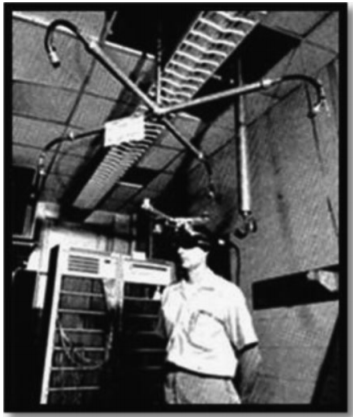
\includegraphics[width=4.5cm]{sutherland.png}
\caption{The Sword of Damocles, by Ivan Sutherland \cite{sutherland}}
\end{figure}
\newline
Since then, driven by the innovation hype, many new AR applications have been invented, not only for entertainment but also for military, medical, and educational purposes. 
\newline
"The Super Cockpit" for instance, invented in the late 1960s, was one of the first AR applications used by the military and a forerunner of the head-up displays still used by fighter pilots today. Sensors attached on the aircraft provided the pilot with visibility in areas occluded by the aircraft structure and by superimposing flight data into the pilot's visual field, superior spatial awareness.\footnote{According to (Mark A. Livingston et al. 2011, Pages 676, 677) \cite{livingston}}
\newline
A more recent application by N. Wake and A. Rosenkrantz empowers the making of AR kidney and prostate malignancy models, giving superior surgical planning, system practice, student training, and patient instruction. Not only does this kind of AR application help patients in an educational sense, it further leads to more precise surgical planning and is therefore of importance for the medical field.\footnote{According to (N. Wake and A. Rosenkrantz 2019, Pages 1, 3) \cite{wake2019}}
\newline
There are also educational applications for AR, like the one invented by I. Dave et al. 
With this AR application, chemistry experiments can be performed in an AR environment, by creating virtual laboratory utensils and chemicals as 3D AR content for this task, which the user can interact with.\footnote{According to (I. Dave et al. 2019, Pages 393, 394) \cite{chemistry}}
\newline
AR even has entertainment potential, like the invention of the game Pokemon GO demonstrated in 2016. It became one of the most successful mobile AR games and reached a mainstream status at that time.\footnote{According to (J. Paavilainen 2017, Page 2493) \cite{pokemon}}
\newline
Like the above instances show, AR has much potential, being able to be used in a lot of different fields, as well as to create different kinds of AR content.
However, it is still facing many challenges, and the Gartner Hype Cycle indicates precisely that.
Every year a research company called "Gartner" evaluates and classifies emerging technologies inside a so-called "Hype Cycle" differentiating what is commercially viable and what is not. The Hype Cycle is a representative of the current life cycle of technologies divided into the stages Technology Trigger, Peak of Inflated Expectations, Trough of Disillusionment, Slope of Enlightenment and Plateau of Productivity with a time x-axis and a expectations y-axis.\footnote{According to (J.H. Kloss 2011, Pages 110, 111) \cite{cycle01}}
\newline
The first time AR appeared on the Hype Cycle was in 2005, classified as Innovation Trigger, which means that the commercial viability of the technology is of yet unproven and the expectations are rising due to the innovation hype. Five years later, in 2010, AR reached the Peak of Inflated Expectations, and with that, some companies start investing in AR while many still do not.
By 2013 and since today, AR has been classified to be in the Trough of Disillusionment, which indicates that many companies interest in AR is decreasing steadily and experiments and implementations fail to deliver what they seemed to be promising.\footnote{According to (Gartner Inc 2019) \cite{gartner01}}
\begin{figure}[h!]
\centering
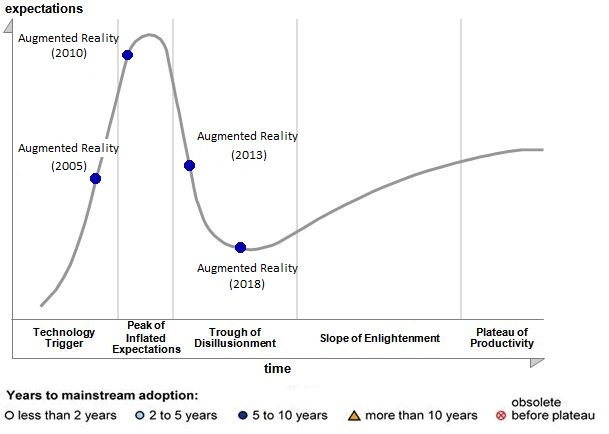
\includegraphics[width=\textwidth]{cycle.jpg}
\caption{Gartner Hype Cycle: Augmented Reality \cite{gartner02}}
\end{figure}
\newline
In my opinion, the decrease of interest in the technology of AR is because the creation of the AR content is a challenging task, both in development effort and development time.
\newline
Whereas AR is widely in use in the medical, military, education, and entertainment fields like mentioned before, the content creation behind this technology is most of the time still done manually. In other words, AR environments are put together by hand without any automation behind it, which will result in higher costs for the consumers of AR apps and higher complexity of the development process. Expensive AR applications, may not be a significant drawback in more rich fields like the military since it is still frequently used there, but it makes AR technology unaffordable for most companies, which is unacceptable in a commercial sense.
Particularly the automation of the development process of said AR applications is of significant importance since it is the main cost factor.
Therefore, this bachelor thesis pursues to design and build a framework, that automates the creation of AR content, reducing development effort and development time, and thus reducing the resulting development costs.
\newline
Speaking of content creation, in this sense, describes the process of creating immersive artificial elements, which can be augmented into a real-world environment and with which the user can interact.
Automation, in this sense, refers to the creation of an adaptable framework that is capable of creating AR content from different types of content. 
To accomplish the automatization of AR content creation, this bachelor thesis introduces a framework, following the approach of automatically generated walkable graphs in an AR environment and with that taking a step in the direction of automatized AR content creation with the use of \ac{ML} techniques.

%%% RESEARCH QUESTIONS %%%
\subsection{Research Question}
Since the examination into AR has so far, for the most part, been focusing on creating handmade AR content, promoting and encouraging the development of AR content in an automatized way, be that as it may, is as yet a substantially less examined area.
Moreover, since the content creation is the fundamental aspect of the automation process, these concerns lead to the following research question:
\begin{itemize}[leftmargin=2cm]
    \item [\textbf{RQ:}] How can the content creation for AR applications be automated?
\end{itemize}
Content means here, in particular, walkable virtual graphs. 
Walkable graphs are artificially created graphs, consisting of edges and nodes, laid on the floor, which can be walked on by the user of the AR application.
They are further capable, to capture and connect all kinds of virtual content such as images, videos, text, 3D elements, and more.
Concerning the research question defined above, the following hypothesis needs to be investigated:
\begin{itemize}[leftmargin=2cm]
    \item [\textbf{H:}] Using parametrization techniques for automating the content creation of virtual graphs will result in a reduction of the needed resources for the development of AR-based walkable graphs than manually extracting and creating content for AR applications.
\end{itemize}
The mentioned resources are the time, and the effort needed to develop the AR application.
To elucidate the research question, a structure in the form of an AR application for the Microsoft HoloLens will be presented, that pursues to automatize the creation of AR content by generating walkable graphs in a blended reality environment. The content created in this process relies on the information that was extracted out of research papers beforehand.
\newline
Since the extracted information could be divided into three layers, the starting point with the information of the paper, the separation of the references into groups and finally the references themselves, it has offered to use walkable graphs with depth two, while every depth, counting from zero, represents one of the spoken about layers. 
\newline
The depth of a graph is the largest number of edges which need to be crossed to walk from the root to the last node without a successor, of the graph.
The full functionality, design, and requirements will be discussed in the following sections.

%%% RESEARCH GOAL %%%
\subsection{Research Goal}
To give a satisfying answer to the previously specified research question, in the course of this bachelor thesis, right off the bat an overview of existing related work concerning the area of automatized AR content creation needs to be presented, their limitations shown and highlighted. This examination is required to differentiate this thesis from related work and to show that the approach followed goes beyond state of the art.
\newline
After that, the conceptual arrangement of the implementation design and considerations concerning the AR application will be tended to. Finally, the approach should be implemented as an AR application for the Microsoft HoloLens, called "The Walkable Graph," which will be utilized to validate the set hypothesis and with that, give an answer to the research question defined in the previous section. Additionally, in a later section, an evaluation plan will be presented, which can be used as a guideline to evaluate the hypothesis defined in the previous section.

\clearpage
%%% METHODOLOGY %%%
\subsection{Methodology}
In the method spectrum of information systems, there are ten different methods formalized by T. Wilde and T. Hess ordering research standards. These methods can moreover be part by the level of formalization into qualitative and quantitative variations.\footnote{According to (Wilde 2007, Page 282) \cite{wilde}}
My bachelor thesis pursues the "Prototyping" technique, which is a more develop arranged research approach with a qualitative level of formalization since it is a general numerical representable issue. The objective of the Prototyping method is to develop and evaluate a pre-release version of an application framework, which I do by building up an AR application.\footnote{According to (Wilde 2007, Page 284) \cite{wilde}}
\newline
Furthermore, this bachelor thesis is situated on the \ac{DSR} guidelines characterized by Hevner.
The first of them being the "Design of an artifact," which expresses that the DSR must deliver a consistent framework as a build, a model, a method, or an instantiation. On account of this theory, this is the recently referenced implementation that I use as a proof-of-concept prototype for the acknowledgment of automatized AR content creation.\footnote{\label{note1}According to (Hevner 2010, Page 13) \cite{hevner}}
\newline
The second guideline is the advancement of innovation based answers for significant and essential business issues. This guideline is referenced in the motivation section of this thesis, which provides up-to-date information, and addresses current and future issues.  
Concerning the third guideline, an evaluation plan will be presented, and ought to be tended to by a master thesis, later on.
The next guideline, called "Research contributions" demands to provide transparent and verifiable contributions, which I tend to follow by giving scientific references and calculations, if needed for a better understanding, to every written statement. The guidelines called "Research rigor" and "Design as a search process" signify that rigorous methods in both the construction and evaluation of the design artifact and crystalizing constraints of the problem field are of importance. I pursue to follow these guidelines by discussing the approach of the AR application "The Walkable Graph," determining the constraints of the problem field and giving a solution to said constraints, supported by mathematical calculations.\footnoteref{note1}
\newline
In the last guideline, called "Communication of research" Hevner demands to publish and present the design science research, which I will do by publicizing this bachelor thesis in a digital form and finally presenting my work for my bachelor seminar in front of a technology-oriented audience.\footnote{According to (Hevner 2010, Page 13) \cite{hevner}}

%%% THESIS STRUCTURE %%%
\subsection{Thesis Structure}
This bachelor thesis intends to design and build a framework that automatizes AR content creation by utilizing \ac{NLP} and graph generation.
The idea for the AR application was initially created at the DFKI with the help of Springer Nature, as a particular use case for readers of academic publications. A user who peruses a scholarly publication in digital or in printed form would have the possibility to experience further virtual content and to investigate walkable graphs containing data which is specially related with the paper, by using the AR application "The Walkable Graph."
To have the capacity to respond to the research question, develop the referenced framework, and follow the guideline of the Prototype methodology, this bachelor thesis seeks after the following structure:
\newline
The inspiration in section I gives a presentation into the significance of this theme. Section II characterizes the information base and examines related work in the field of AR content creation, discussing the pursued approaches, and investigating their limitations. Section III covers the application setting, the thoughts behind the design decision, and the implementation design.
\newline
Section IV will, at that point, talk about the execution of the AR application, which will be utilized as a proof-of-concept prototype to address the research question and evaluate the hypothesis.
\newline
After that, section V will give an evaluation plan, defining variables that need to be addressed at a later point. At last, section VI wholes up the goals and consequences of the thesis discusses the limitations, viewpoint, and addresses future work in this research area.
\clearpage


%%% RELATED WORKS %%%
\section{Related Work}
This section will introduce the reader with related work, that are of qualitative substance towards this research issue, and their respective approach and concept are therefore being investigated in detail in the following.
An outline of the discoveries follows, for each subchapter, with a portrayal of restrictions and weaknesses of the introduced related work.

%%% AUTOMATED content creation %%%
\subsection{Automated Content Creation}
Automated content creation, in general, describes the process of creating digital content in an automated manner. Automation is accomplished by using different frameworks, that pursue to minimize the time needed to create digital content.
The mentioned digital content can be split into three main categories, 2D (e.g., web design), 3D (e.g., 3D modeling) and 4D (e.g., visual effects) digital content.
\newline
\newline
%%% PRINT MEDIA %%%
The automated content creation of 2D content has been investigated in "Automated AR Content Creation for Print Media," by R. Raso et al. By uniting print media with AR content, the mentioned paper pursues to avert the decrease in print media. Especially the issue of the absence of automation and standardization is being referenced, which is the main factor why the use of AR is decreasing in print media.\footnote{According to (R. Raso et al. 2016, Pages 245, 246) \cite{rocco}}
\newline
To proof the idea of automatized AR content creation, a framework in the form of an AR application is being built, that ensures new reading experiences to the readers of print media. With the integration of a recommender system, individualized suggestions can be given to the user, and potential AR contents are elected automatically, like links to the online version of the newspaper, video sharing websites and social media. \footnote{According to (R. Raso et al. 2016, Pages 250, 251) \cite{rocco}}
\newline
The objective of this paper, was the automation of AR content creation, explicitly for print media, and therefore the limitation concerning this work depends primarily on the fact that it was made for this particular use case. This framework, however, might be adequately stretched out to different alternate paper-based applications in future research works.
\newline
\newline
%%% 3D MODELING %%%
The scientific paper "Virtual Reality and Augmented Reality in Digestive Surgery" by L. Soler et al. investigates the automated creation of 3D content. By using the CT-scans of the patient, the developed system creates 3D models of the anatomical and pathological digestive system of the patient in an automated manner. It enables intraoperative abdominal surgery advancements, like improved surgical planning, and by using simulations, the possibility to train surgical gestures before carrying them out.\footnote{According to (L. Soler et al. 2004, Page 278) \cite{digestiv}}
The 3D models are created automatically, by delineating interior structures out of CT-scans, using AR reference models, and deforming their contours according to the delineations.\footnote{According to (L. Soler et al. 2001, Page 131) \cite{digestiv2}}
\newline
This paper aimed to develop a framework for the 3D modeling of abdominal CT-scans. The limitations of this scientific work are that it has been developed for a specific field of application and that markers need to be stuck to the patient for enhanced precision.\footnote{According to (L. Soler et al. 2004, Page 279) \cite{digestiv}}
\newline
\newline
M. Golparvar-Fard et al. pursued an alternate objective. In "Application of D4AR - A 4-dimensional augmented reality model for automating construction progress monitoring data collection, processing, and communication", which investigates automated 4D AR modeling.
4D modeling is the process of creating 3D models over a fixed period, for a reason to be able to see possible changes of the referenced model.
In this work, 4D AR models of schedules delay in field construction are built using a traffic light metaphor to indicate actual and as-planned performances. \footnote{According to (M. Golparvar-Fard et al. 2009, Page 129) \cite{4D}}
The superimposed models are colored green if they are ahead of schedule, yellow if they are on schedule and red if they are behind schedule. This application can be utilized by project managers to monitor the construction progress.\footnote{According to (M. Golparvar-Fard et al. 2009, Page 137) \cite{4D}}
The 4D models are created by using time-lapse photography, that is used in computer vision techniques to compute the models. Furthermore, the as-planned model is superimposed, and the traffic light metaphor is applied to the model..\footnote{According to (M. Golparvar-Fard et al. 2009, Page 139) \cite{4D}}
\newline
\newline
The limit concerning this paper relies on the fact that it depends on good quality time-lapsed photography, which is not always given, especially in unfavorable weather situations. In the case of interior construction progress monitoring, many cameras in every room would be needed to get the time-lapse photography needed.
\newline
\newline
"Augmented Reality Authoring: Generic Context from Programmer to Designer" by  A. Hampshire et al. introduces a framework, that allows the developer to implement AR applications more rapidly by utilizing a higher level of abstraction. The goal of this thesis was to build a framework called OSGART, that generalizes common aspects and generalizes meta structures, hence becoming a tool, that can be used for rapid development of AR prototypes.
The tool was evaluated by an actual academic project and has shown that it reduces the development time and effort for AR applications.\footnote{According to (A. Hampshire et al. 2006, Pages 409 - 412) \cite{frameworkAutomation}}
By using a higher level of AR-content abstraction, A. Hampshire et al. have shown a way to automate the creation of AR content.
\newline
\newline
By examining other research papers, and their approaches, that are firmly identified with this thesis, I can guarantee that this thesis pursues an alternate approach. Hence, building a framework that can automatize the generation of graphs in an AR environment, this procedure goes past state of the art.

%%% GRAPH GENERATION %%%
\subsection{Graph Generation}
Since the focal piece of this theory is the achievement to produce walkable graphs in an AR domain in an automized way, this segment seeks after to introduce the reader into specific procedures utilized for the graph generation process.
\newline
Since the following explanations refer to graphs and their properties, I will define them in advance.
\newline
A graph when all is said in done represents a set $G = (V, E)$, where $V$ is the arrangement of vertices or nodes, and $E \subset V\times V$ is the arrangement of edges, every one of these edges associating two distinctive vertices. The nodes of a graph can be further divided into root nodes - nodes without predecessor nodes, leaf nodes - nodes without successor nodes, and inner nodes.
\newline
Speaking of isometry, two graphs $G_1$ and $G_2$ are referred to as isometric to each other, if there is a bijection $f: V_{G_1} \longrightarrow V_{G_2}$ between the vertex set $V_{G_1}$ of $G_1$ and $V_{G_2}$ of $G_2$, in such a way, that any two vertices $v_1$ and $v_2$ of $G_1$ are on the same edge in $G_1$ if and only if $f(v_1)$ and $f(v_2)$ are on the same edge in $G_2$.
\newline
Furthermore, a planar graph denotes a graph without edge and node intersections.
\newline
\newline
%%% TREE GRAPH GENERATION %%%
"A Survey Of Graph Generation Techniques" by Ronald C. Read, shows an assortment of graph generation techniques that are used to make graphs with specified properties.
In the first place, the peruser is acquainted with old strategies for graph generation, where the quantity of graph vertices is set as the target property of the graph. 
In the precedent with four vertices, edges are added to the vertices in every conceivable blend to create graphs of four vertices.
During the time spent to structure those graphs, the isometric ones are filtered out, to avoid duplicate graphs of the equivalent structure.\footnote{According to (R. Read 1981, Page 77) \cite{graphGen}}
\newline
To have the option to decide whether two graphs are isometric or not, some code is needed to represent the graph structure, while each structure ought to have its extraordinary code. On account of graphs with a tree-like structure, this is done by walking around the tree in a clockwise direction and noting zero if the node is a leaf node and, one, else. This methodology is delineated in the following picture.\footnote{According to (R. Read 1981, Page 82) \cite{graphGen}}
\begin{figure}[h!]
\centering
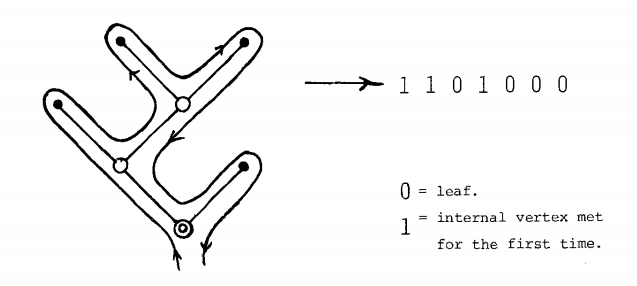
\includegraphics[width=7cm]{graphGen.png}
\caption{Graph Generation: Isometry Code \cite{graphGen}}
\end{figure}
\newline
The limitations regarding these graph generation techniques rely on the absence of property alterations. Like expressed later in the implementation area, I seek to make a planar graph that has a symmetric structure and that for each group and node amount has a close ideal arrangement.
\newline
The referenced paper pursues an alternate objective and does not focus on said planar graphs; the objective here is the generation of graphs that can be produced by the recently made list of graphs, of the previous iteration while filtering the isometric ones through.
\newline
\newline
%%% RADIAL GRAPH GENERATION %%%
By producing so-called radial graphs, "Radial Level Planarity Testing and Embedding in Linear Time*" by C. Bachmeier et al., follows an alternate approach.
Outspread, spiral or radial graphs are like regular graphs, yet the nodes and edges are orchestrated concentrically. Besides, the goal of the introduced paper is to build these graphs to be planar.
A graph with a given parceling of its vertices onto $k$ concentric circles is $k$-radial planar if the edges can be directed monotonic between the circles without intersections.\footnote{According to (C. Bachmeier et al. 2004, Page 393) \cite{radialgraph}} 
\newline
The underlying algorithm used, can compute the radial planar graph in linear time and tries to minimize edge crossings, while doing so, the best case is not to have any crossings at all. The said algorithm does so, by partitioning the vertex set $V$ into $k$ subsets $V_1, ..., V_k$, where each vertex $v$ of different subsets is placed on different concentric circles and the edges are drawn in monotone curves without crossings.\footnote{According to (C. Bachmeier et al. 2004, Pages 393, 394) \cite{radialgraph}}
While related works pursue to place the vertices on k horizontal lines, this one does on $k$ concentric circle lines. Since every planar graph can have a k level planarity, if the edges are arbitrarily long enough, which can be seen in the later implementation section, this paper gives a solution for every given $k$.\footnote{According to (C. Bachmeier et al. 2004, Page 394) \cite{radialgraph}}
\newline
A three-radial planar graph is practically what the walkable graph could use since the point of view would be a representant of the primary dimension, the group node the representant of the second dimension and the paper node for the third dimension. Moreover, planarity would be given, with the end goal that none of the nodes and edges would meet one another, which is alluring too.
\newline
However, the concentric edges would be confusing for the user to walk on, and the objective of the presented paper was not focused on the place management issue, which I talk about in a later chapter. The still pretty effective technique showed in this paper, is delineated in the following picture.

\begin{figure}[h!]
\centering
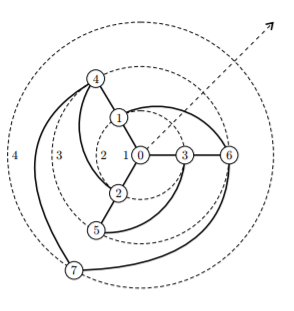
\includegraphics[width=5cm]{radial.png}
\caption{Radial Graph, by C. Bachmeier et al. \cite{radialgraph}}
\end{figure} \par


%%% USER IN MOTION MR %%%
\subsection{User In Motion MR}
This subchapter investigates MR applications where the user is expressly in movement.
To be more precise, the term User in Motion MR describes the process by which the user of an MR application finds himself walking, in an MR environment, and interacting with possible virtual content.
MR, in this differentiation, is being limited to AR and VR environments exclusively. In the following two applications are presented, compared, and potential issues that could occur while walking in MR environments talked about. The first of them taking place in an AR environment and the other in a VR environment.
\newline
\newline
%%% USER IN MOTION AR %%%
One of the issues concerning AR are environments, which include walking onto virtual paths on the floor. 
These specified AR environments have been investigated in the work "Walking in Augmented Reality: an experimental evaluation by playing with a virtual hopscotch" by M. Chessa and F. Solari, in which non-prepared individuals were approached to play with a virtual hopscotch.\footnote{According to (M. Chessa and F. Solari 2017, Page 143) \cite{arhopscotch}}
\newline
Hopscotch is a game for young people, where the goal is, to jump over a numbered way drawn on the floor.
Much the same as in my thesis, this paper follows the prototyping methodology and uses an AR application for evaluation reasons. The assessment process consists of two sections, the self-assessment questions and the capturing of the 3D positions of the paths walked on by the user, which provide information about possible errors that occurred, when looking at the design of the hopscotch.
A picture of the AR hopscotch is shown in the following.\footnote{According to (M. Chessa and F. Solari 2017, Pages 143, 144) \cite{arhopscotch}}
\begin{figure}[h!]
\centering
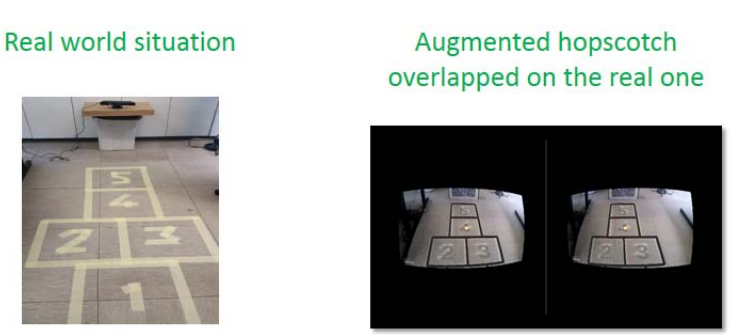
\includegraphics[width=9cm]{hopscotch.png}
\caption{Walkable AR Hopscotch, by Chessa and Solari \cite{arhopscotch}}
\end{figure}
\newline
Amid the test, the users were approached, to hop the hopscotch and later on to answer inquiries for assessment reasons. The users were wearing HMD's, which are necessary for this task since the user needs to be able to move more naturally and for this reason, be freehanded. The result of this assessment part demonstrated that individuals who pursued a virtual way overlaid on the original floor, in an AR environment, experienced misperception issues. Specifically, it was demonstrated that the evaluated participants pursued a shorter and twisted way instead of the structured one. The mistake in the perception of the way achieved roughly nine percent.\footnote{According to (M. Chessa and F. Solari 2017, Page 147) \cite{arhopscotch}}
\newline
However, by utilizing a more up to date model AR device like the Microsoft HoloLens, a diminishing of the path perception error is expected, due to fresher advancements being utilized for the posture estimation. Even if there is no improvement of the perception by utilizing the HoloLens, an error of around 10\% won't influence the application of the Walkable Graph, since the ways on the floor being utilized don't necessarily need to be walked on, they only have the task, to direct the client to the following group or paper nodes.
\newline
\newline
%%% WALKING IN VR %%%
The paper "Building a memory palace in minutes" by Eric Legge et al. pursues the idea, to develop a walkable memory palace in a VR environment as a VR application. The memory palace, also called the \ac{MOL}, is a method used to enhance memory. By visualizing information in an environment, it empowers the user to recall data all the more rapidly and productively.
Explicitly this paper validates how user-friendly the VR concept is, whether it improves the user's memory in remembering an ordered list of items and if any alternations of virtual environments have a more effective outcome in that procedure.
The conventional MOL method in a familiar environment, called cMOL, is being differentiated to the virtual environment technique, called vMOL.\footnote{According to (Eric Legge et al. 2012, Pages 380, 381) \cite{mempalace}}
\newline
The results of the assessment procedure of the application demonstrated that members of the vMOL method were compliant for 58.8\% of records and the cMOL strategy 44.8\%, while both the procedures had a similar effect to the memory enhancement. \footnote{According to (Eric Legge et al. 2012, Page 383) \cite{mempalace}} 
The outcomes show further that profoundly conceivable words are reviewed more precisely than theoretical words. \footnote{According to (Eric Legge et al. 2012, Pages 385, 386) \cite{mempalace}} 
\newline
The following picture depicts the application discussed:
\begin{figure}[h!]
\centering
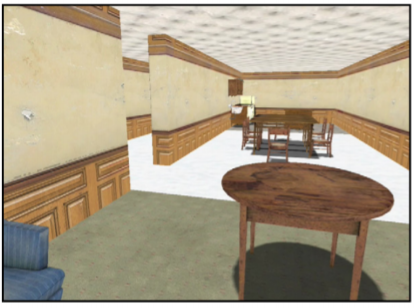
\includegraphics[width=7cm]{mempalace.png}
\caption{VR Memory Palace, by Eric Legge et al. \cite{mempalace}}
\end{figure}
\newline
The results demonstrate that vMOL and cMOL both improve the MOL procedure in recalling word lists; therefore, a mix of both procedures, by utilizing AR could upgrade the method considerably further. Since the AR application "The Walkable Graph" can be utilized to play out the MOL in a particular and well-known environment while the user can interact with the AR content, it very well may be more precise than the cMOL or vMOL strategy exclusively. This hypothesis ought to be researched and taken into consideration in the later evaluation plan.

%%% AR INTERFACE %%%
\subsection{AR Interfaces}
An interface is used by humans to facilitate interactions with software or hardware components. For the prototype "The Walkable Graph" an interface is needed, that for once, enables the user to see the AR content melded into the surroundings, and also enables the user to walk around and interact with the displayed AR content. Especially the later evaluation, which is needed to proof the set hypothesis, makes the choice of the right AR interface important.
\newline
\newline
A subsection of the work "A Survey of Augmented Reality" by M. Billinghurst, called "AR Input and Interaction Technologies" investigates AR interfaces in more detail. AR interfaces can be split into five categories, namely Information Browsers, 3D User Interfaces, Tangible User Interfaces, Natural User Interfaces, and Multimodal Interfaces.\footnote{According to (M. Billinghurst et al. 2015, Pages 165, 166) \cite{interfaces}}
These categories are discussed, and examples of AR interfaces to each respective category are named in the following.
\newline
AR information browsers are interfaces with which the user can see AR content on display, may it be hand-held or head-worn. Interactions with these kinds of interfaces are limited to a regular 2D \ac{GUI}, and by moving the interface about the environment, AR content placed into the environment can be seen. A prominent AR information browser, is the hand-held device called NaviCam invented by Nekimoto and Nagao in 1995.\footnote{According to (M. Billinghurst et al. 2015, Pages 166, 167) \cite{interfaces}}
\newline
3D User Interfaces for AR can be utilized to interact with virtual content by using controllers directly. These controllers track the motion of the user and with that, enable the user to interact with AR and VR content. An example of such an interface is the haptic device called phantom.
\footnote{According to (M. Billinghurst et al. 2015, Pages 167, 168) \cite{interfaces}}
\newline
Tangible User Interfaces use physical objects to interact with virtual content. Each virtual content is placed on a physical object and said virtual content could be manipulated by manipulating the respective physical object. While Tangible User Interfaces provide intuitive interaction with virtual content, they have display capability limitations. An example of tangible based interfaces are paper cards, which have markers printed on them, and which trigger virtual content to be created on top of those cards. \footnote{According to (M. Billinghurst et al. 2015, Pages 170, 171) \cite{interfaces}}
\newline
Natural User Interfaces are interfaces that can track body motion and recognize gestures. The user can interact with virtual content by performing gestures in front of the sensors of the AR interface. An example of such an AR interface is the Microsoft HoloLens.
\footnote{According to (M. Billinghurst et al. 2015, Pages 172, 173) \cite{interfaces}}
\newline
Multimodal Interfaces provide richer interactivity, like speech and gesture recognition. They allow intuitive interactions with virtual content, speech for quantitative, and gesture for qualitative input. Again, the Microsoft HoloLens is a representant thus it enables the user to interact with AR content by speech and gestures.\footnote{According to (M. Billinghurst et al. 2015, Pages 175) \cite{interfaces}}
\newline
Since the AR prototype "The Walkable Graph" needs the user to be in motion, exploring the AR content on a walkable graph and interacting with it, a multimodal interface like the Microsoft HoloLens is a perfect fit. That is why I decided to use the Microsoft HoloLens for prototype development.

\begin{comment}
A \ac{SDK} is a collection of software that can be used by the programmer to develop specific applications. Identifying the best-fitting SDK for the development of the proof-of-concept prototype "The Walkable Graph" is of essential importance, and likewise is the device being used for the development and later evaluation process.
\newline
\newline
%% DEVICE %%%
The first paper I am introducing is called "Comparison of optical see-through head-mounted displays...", by Long Qian et al.
Three commercially available devices that are representative for the current state HMD's are being contrasted, expressly ODG R-7, the Epson Moverio BT-200 and the Microsoft HoloLens.\footnote{According to Long Qian et al., Page 901\cite{devices}}
\newline
The mentioned HMD's are being evaluated in contrast to text readability, contrast perception, task load, frame rate, and system lag.\footnote{According to Long Qian et al., Page 901, 902\cite{devices}}
The result of this evaluation showed that the HoloLens outperforms the other two HMD's in almost every rubric tested. Specifically, in perception, task load, and framerate, the HoloLens performs more efficiently, resulting in a significantly smaller system lag.
Regarding text readability the HoloLens goes on par with the R-7.\footnote{According to Long Qian et al., Page 908\cite{devices}}
\newline
The outcomes demonstrate that the wearable gadget  was seen to be increasingly precise and along these lines urges us to have settled on the correct decision, picking the Microsoft HoloLens for the AR application "The Walkable Graph."
\newline
\newline
%%% SDK %%%
Since I settled down to use the Microsoft HoloLens as the device of choice, I now have to pick a fitting SDK.

There are several SDK's that are being created and improved for the utilization of AR programming, such as the ARKit (Apple) and ARCore (Google), which are probably the most perceived ones.
\newline
Since the proof-of-concept prototype of this proposition is being programmed with the assistance of Unity and for the AR device, Microsoft HoloLens, an SDK needs to be chosen that fits these extraordinary needs the best.
\newline
The work I inspected acquaints the peruser with 12 AR SDK's that are as of now being utilized the most. Almost every one of them, except for ARCore and Wikitude, explicitly named to have Unity support. Onirix and the \ac{MRTK} even name the HoloLens individually as a supported gadget and are for this reason the most likely best choice for an SDK.\footnote{According to Dzone\cite{sdks}}
\newline
The motivation behind why I finally picked the MRTK SDK is that it is the most recommended SDK by Microsoft. It enables me to have a HoloLens ideal SDK, pre-made prefabs, and spatial processing, which I require for the advancement procedure of the prototype "The Walkable Graph."
\end{comment}

\clearpage
%%% APPROACH %%%
\section{Approach}
In this segment, the methodology and the structure of the prototypical implementation of the recently referenced AR application called "The Walkable Graph" will be talked about. I am starting with the clarification of the idea itself and the elucidation of essential rules that are put into the plan and advancement of this application, trailed by the constraint assurance and calculations required for the space management of the computed AR Content.

%%% CONCEPT %%%
\subsection{Concept}
The application that was intended to prove the hypothesis that automation of AR content creation is, in reality, conceivable, is an AR application for the Microsoft HoloLens. It tends to a particular use case for perusers of scholarly publications, empowering them to investigate walkable graphs containing additional data specifically related to the publication, by means for an AR interface.
\newline
Each academic paper contains a list of references, which are fundamental for the appreciation of the research work and are utilized to prove logical statements and proclamations. As per their examined theme, these references can be additionally clustered into groups of references. The referenced references and their groups would then be able to be used to build up a graph with depth two in an AR environment. This graph can further be improved with data of virtual substance, for example, abstracts, keyword list, SciGraph's and considerably more, and be gone through by the peruser in an AR domain.\footnote{According to (R. Raso et al. 2019, Pages 3, 4) \cite{walkable}}
\newline
To empower the automated generation of walkable graphs for reference grouping a research team at the DFKI in Saarbrücken built up a framework,
in cooperation with Springer Nature, comprising of four principal parts which are the base of my prototypical implementation.
\newline
The main parts of the underlying software architecture are the External Applications, the Extract Backend Engine, the Data Layer, and the HoloLens application. The purpose of the Knowledge Extraction Part it is, to extract data out of scientific papers by using External Applications like the Springer Nature, SciGraph, Citation \ac{API}'s and \ac{NLP}, which is a common \ac{ML} technique to be used for such a task. 
The resulting extracted data is then being stored in the form of an XML file in the Data Layer.
An API is an interface that enables program connections at the source-code level, for example, to grant access to databases. The ML technique used here, namely NLP, will be clarified in detail later on.
\newline
Furthermore, with the use of an AR Interface Development System, the XML file representing a particular paper can be retrieved from the Data Layer, by gathering all essential data needed, to characterize the final structure of the walkable graph. The result finally gets forwarded to the HoloLens application, where the graph is being rendered, and the extracted data is presented as AR content in an AR environment in the form of a walkable graph.\footnote{According to (R. Raso et al. 2019, Page 4) \cite{walkable}}
\begin{figure}[h]
\centering
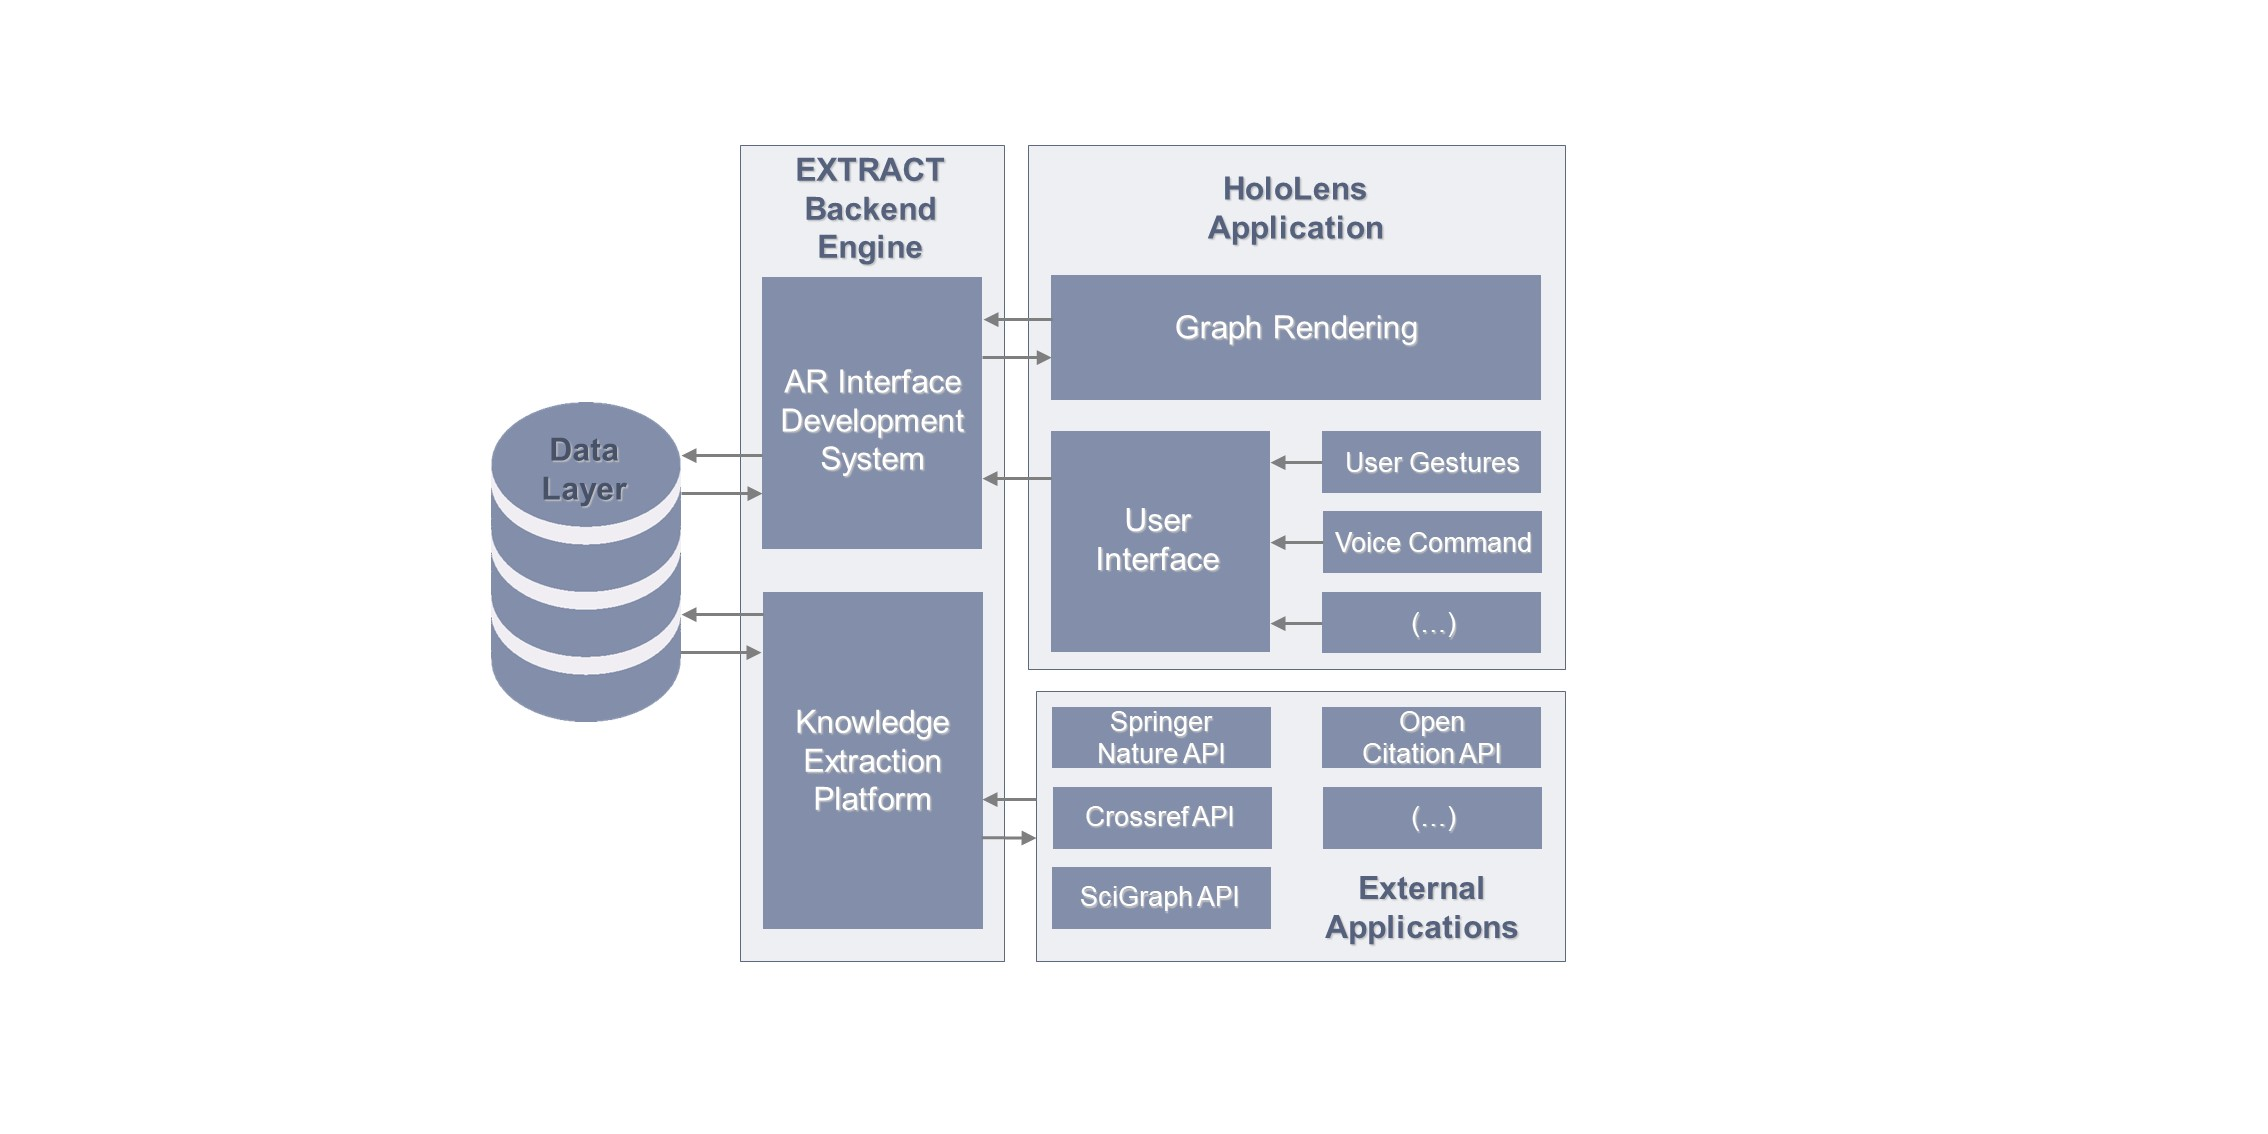
\includegraphics[width=\textwidth]{Arch.jpg}
\caption{The Walkable Graph: Software Architecture \cite{walkable}}
\end{figure}
\newline
The number of groups and their particular references characterize the structure of the graph as well as the constraints that will be defined in the following sections. The following figure demonstrates a flexible structure of the walkable graph as an AR picture seen from the HoloLens, which represents the final product conceptually.
\clearpage

\begin{figure}[h]
\centering
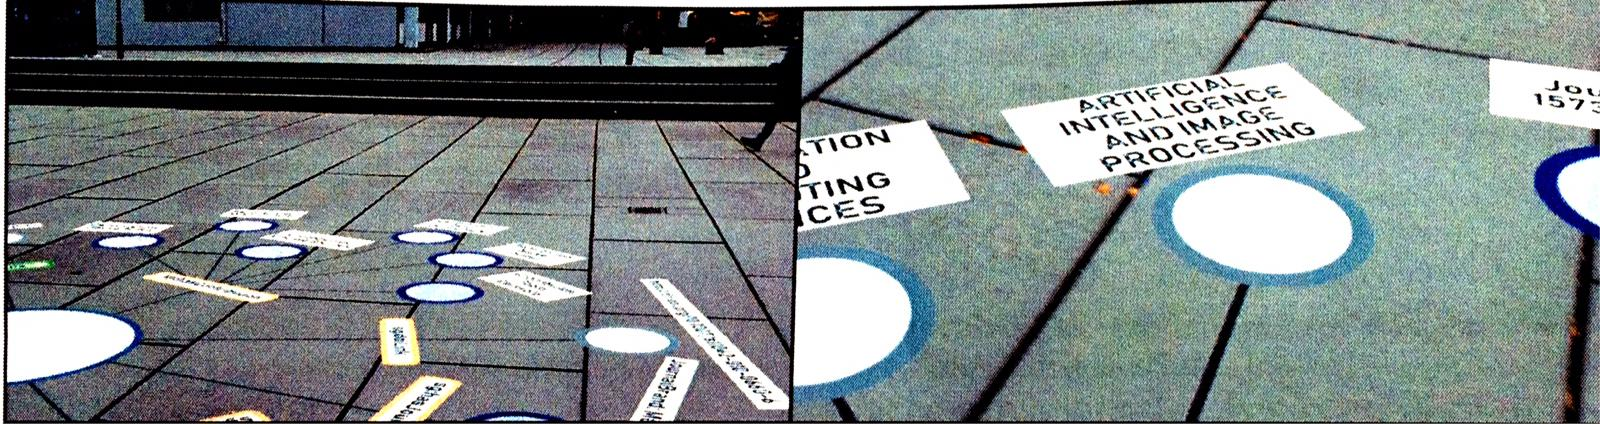
\includegraphics[width=\textwidth]{WalkableGraph.jpg}
\caption{The Walkable Graph: Concept Image \cite{walkable}}
\end{figure} \par

%%% DESIGN PROCESS %%%
\subsection{Design Process}
The design procedure of the recently referenced AR application called "The Walkable Graph" can be part into three subcategories, to be specific workflow, procedure, and the process of information acquisition.
\newline
Everything begins with a paper $\phi$ from which a list of n references $P_1, .., P_n$ are extricated. In the interim a database is being created with the extricated references list, the keywords of each paper and their abstract put away for later use. Besides, the references are clustered to groups according to their inspected theme by the utilization of an ML technique called NLP.
To deliver noteworthy bits of knowledge from content information, here scientific paper, and to open the capability of content information, NLP is utilized. NLP is the procedure to make human language interpretable for machines.\footnote{According to (A. Kulkarni and A. Shivananda 2019, Pages 17, 18) \cite{NLP}}
\newline
These means consolidated the recently referenced "Knowledge Extraction," which yields a vector of information, containing among other data, reference list and groups of references for every single accessible item of the dataset.\footnote{According to (R. Raso et al. 2019, Page 4) \cite{walkable}}
After that, the procedure of the VR Model Preparation starts, which is a piece of the as of late referenced "AR Interface Development System."
\newline
By querying the results of the clustering procedure, the VR model can be readied, gathering fundamental graph building data like what number of groups there are, what sort of group highlights exist and which references are identified with which group. These data are necessary to construct the edges of the graph. Besides, by querying the already made database data like what the virtual content ought to appear every node, what sorts of nodes exist and which node activities ought to be accessible can be extracted. These data are necessary to construct the nodes of the graph, and together with the edge data, the graph itself can be assembled.\footnote{According to (R. Raso et al. 2019, Page 4) \cite{walkable}}
\newline
Having all the data that is required for the walkable graph to be created, the procedure of the VR Model Building can begin. After querying the VR model arrangement data, the VR Model Building process needs to characterize constraints and esteem relationship to have the capacity to create the AR application "The Walkable Graph." 
In the following subsections, the VR Model Building process and the characterized constraints will be talked about in more detail.

%%% VR MODEL BUILDING %%%
\subsection{VR Model Building}
The data queried from the VR Model Preparation process should be put away in some directory to be accessible for the AR application that will be worked for the Microsoft HoloLens, called "The Walkable Graph."
\newline
Therefore, the data, containing the number of groups, the number of nodes in each group separately and the extra node data about the referenced papers are put away in an XML record which can be opened from the HoloLens at runtime. The AR application was built to handle both XML and JSON records.
These record formats were picked without the confinement of any sort since they are the most popular file formats picked for data stockpiling and recovery.
The XML documents made by the NLP technique in the "Knowledge Extraction" process are of the following structure:
\newline
\begin{lstlisting}[basicstyle=\tiny, caption={The used XML Scheme}]
<xs:schema attributeFormDefault="unqualified" elementFormDefault="qualified" xmlns:xs="http://www.w3.org/2001/XMLSchema">
  <xs:element name="WalkableGraph">
    <xs:complexType>
      <xs:sequence>
        <xs:element name="PaperInfo">
          <xs:complexType>
            <xs:sequence>
              <xs:element name="Paper">
                <xs:complexType>
                  <xs:sequence>
                    <xs:element type="xs:string" name="DOI"/>
                    <xs:element type="xs:string" name="Abstract"/>
                    <xs:element type="xs:string" name="Authors"/>
                    <xs:element type="xs:string" name="Keywords"/>
                    <xs:element type="xs:string" name="Title"/>
                    <xs:element type="xs:string" name="Typology"/>
                    <xs:element type="xs:string" name="Year"/>
                    <xs:element type="xs:string" name="SciGraph"/>
                    <xs:element type="xs:string" name="NewOrigin"/>
                  </xs:sequence>
                  <xs:attribute type="xs:string" name="name"/>
                </xs:complexType>
              </xs:element>
            </xs:sequence>
          </xs:complexType>
        </xs:element>
        <xs:element name="Groups_Ref">
          <xs:complexType>
            <xs:sequence>
              <xs:element name="Group" maxOccurs="unbounded" minOccurs="0">
                <xs:complexType>
                  <xs:sequence>
                    <xs:element name="Paper" maxOccurs="unbounded" minOccurs="0">
                      <xs:complexType>
                        <xs:sequence>
                          <xs:element type="xs:string" name="DOI"/>
                          <xs:element type="xs:string" name="Abstract"/>
                          <xs:element type="xs:string" name="Authors"/>
                          <xs:element type="xs:string" name="Keywords"/>
                          <xs:element type="xs:string" name="Title"/>
                          <xs:element type="xs:string" name="Typology"/>
                          <xs:element type="xs:string" name="Year"/>
                          <xs:element type="xs:string" name="SciGraph"/>
                          <xs:element type="xs:string" name="NewOrigin"/>
                        </xs:sequence>
                        <xs:attribute type="xs:string" name="name" use="optional"/>
                      </xs:complexType>
                    </xs:element>
                  </xs:sequence>
                  <xs:attribute type="xs:string" name="name" use="optional"/>
                </xs:complexType>
              </xs:element>
            </xs:sequence>
          </xs:complexType>
        </xs:element>
      </xs:sequence>
    </xs:complexType>
  </xs:element>
</xs:schema>}
\end{lstlisting}
As can be seen from the XML scheme over, a few data could be extracted from the scientific paper.
At the base of the XML document is the walkable graph. The graph speaks to the original paper containing the PaperInfo and Group\_Ref. The Group\_Ref component is the root component of the list of group's of references, and the referenced PaperInfo is the root component of a reference paper.
\newline
Moreover, the Group component is part of a list of reference papers and has a name as a property. All the recently referenced elements are expected to assemble the structure of the graph, and the last component called paper contains all information that needs to be displayed as AR content for the user of the AR environment. The Paper component contains together with its name property the accompanying data:
\newline
\begin{itemize}
\item{\textbf{\underline{DOI}}: DOI is an acronym for "digital object identifier." it is used for a system that provides an infrastructure for appropriate persistent identification of objects of any kind.\footnote{According to DOI Handbook, Introduction \cite{doi}}}
\item{\textbf{\underline{Abstract}}: The Abstract is a synopsis of the referenced paper.}
\item{\textbf{\underline{Authors}}: The authors of the referenced Paper.}
\item{\textbf{\underline{Keywords}}: Keywords are words that capture the quintessence of the paper. Keywords make a document searchable and guarantee to induce more citations.}
\item{\textbf{\underline{Title}}: The title of the referenced Paper.}
\item{\textbf{\underline{Typology}}: Typology most regularly classifies Papers by certain commonalities or ranks them by specific contrasts. Utilizing typology makes a difference for analysts and others to understand specific conditions or variables better.}
\item{\textbf{\underline{Year}}: The Year when the referenced paper was distributed.}
\item{\textbf{\underline{SciGraph}}: The SciGraph interlinks high-quality metadata from Springer Nature and other scholarly partners. It is a visualization of the relationship of connected datasets.}
\item{\textbf{\underline{NewOrigin}}: The NewOrigin is the title of the XML record for the referenced Paper. It is utilized to compute a new walkable graph containing all the above data for the referenced paper.}
\end{itemize}
But not all these components are compulsory, a few of them are optional. To be more precise, the following table summarizes the XML structure in a simplified way, noticing the optional components:
\clearpage
\begin{table}[h]
\centering
\caption{XML Scheme Root, Elements and Attributes}
\begin{adjustbox}{max width=\textwidth}
\begin{tabular}{|l|l|} 
\hline
\textcolor[rgb]{0.2,0.2,0.2}{\textbf{Root}}  & \textcolor[rgb]{0.2,0.2,0.2}{\textbf{Elements}}                                                                                                             \\ 
\hline
\textcolor[rgb]{0.2,0.2,0.2}{Walkable Graph} & \textcolor[rgb]{0.2,0.2,0.2}{PaperInfo, Group\_Ref}                                                                                                        \\ 
\hline
\textcolor[rgb]{0.2,0.2,0.2}{Group\_Ref}     & \textcolor[rgb]{0.2,0.2,0.2}{Group (List)}                                                                                                                  \\ 
\hline
PaperInfo                                    & Paper                                                                                                                                                       \\ 
\hline
Group                                        & Paper (List), name (Attribute)                                                                                                                             \\ 
\hline
Paper                                        & \begin{tabular}[c]{@{}l@{}}DOI, Abstract, Authors, Keywords[?], Title, Typology[?]\\ Year, SciGraph[?], NewOrigin, name (Attribute)\end{tabular}  \\ 
\hline
\textbf{Additional Info}                     & {[}?] := optional Data \textbar{}\textbar{} Encoding used: UTF-8                                                                                             \\
\hline
\end{tabular}
\end{adjustbox}
\end{table}


%%% INFORMATION PROCESSING %%%
\subsection{Information Processing}
Like referenced before, the AR application, "The Walkable Graph" is being created for the Microsoft HoloLens. The most conventional \ac{IDE} used for this task is Unity, and the code to manage the events happening in the application is written in the programming language C\#. I will discuss Unity and other programming utils in more detail later on in the "Tools" section of this thesis.
\newline
To have the possibility to access the XML record of the above-described structure, they must be put into an exceptional folder onto the HoloLens called "StreamingAssets."  I am using this folder since it is the primary resources folder in Unity, which gets replicated over to the HoloLens without making changes on the files or compressing them.
There exist other reasonable answers for this issue, which would work as well, for instance, the XML file could be loaded as a URL instead.
The first thing the user finds in the wake of starting the application "The Walkable Graph" is a menu that engages the user to pick a specific XML report through a dropdown. The dropdown contains all XML records that are contained in the "StreamingAssets" folder. The chose scientific paper can, from that point onward, be computed as a walkable graph by pushing on the corresponding button.
\clearpage
\begin{figure}[h!]
\centering
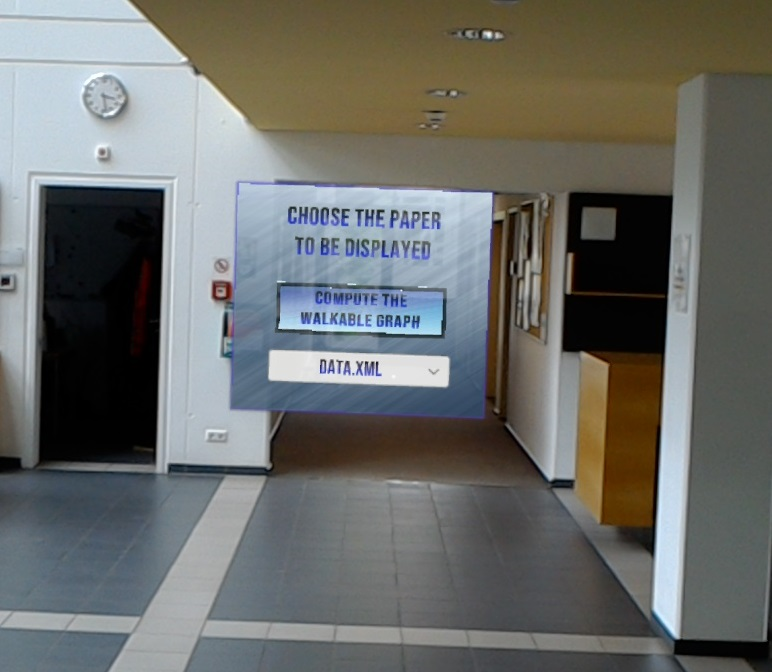
\includegraphics[width = 10 cm]{menu2.jpg}
\caption{The Walkable Graph: Startmenu}
\end{figure} \par
To get the XML files to be converted into useable C\# objects, the chosen XML record has to be deserialized. Deserialization is the way toward interpreting XML documents into C\# objects by giving it the structure of the XML, which can be found in the past table, to a function contained in the "System.XML" bundle. A code piece of this procedure is shown in the following:

\begin{lstlisting}[basicstyle=\tiny, caption={XML Deserialization, C\# Code Snippet.}]
    [Serializable()]
    [XmlRoot("WalkableGraph")]
    public class WalkableGraph
    {
        [XmlElement("PaperInfo")]
        public PaperInfo PaperInfo  {get; set; }

        [XmlElement("Groups_Ref")]
        public Groups Groups        {get; set; }
    }

    [Serializable()]
    [XmlRoot("Groups_Ref")]
    public class Groups
    {
        [XmlElement("Group")]
        public List<Group> Group    {get; set; }
    }
    
    [Serializable()]
    [XmlRoot("Group")]
    public class Group
    {
        [XmlElement("Paper")]
        public List<Paper> Paper    {get; set; }

        [XmlAttribute("name")]
        public string GroupName     {get; set; }
    }

    [Serializable()]
    [XmlRoot("PaperInfo")]
    public class PaperInfo
    {
        [XmlElement("Paper")]
        public Paper Paper          {get; set; }
    }

    [Serializable()]
    [XmlRoot("Paper")]
    public class Paper
    {
        [XmlElement("DOI")]
        public String DOI           {get; set; }

        [XmlElement("Abstract")]
        public String Abstract      {get; set; }

        [XmlElement("Authors")]
        public String Authors       {get; set; }

        [XmlElement("Keywords")]
        public String Keywords      {get; set; }

        [XmlElement("Title")]
        public String Title         {get; set; }

        [XmlElement("Typology")]
        public String Typology      {get; set; }

        [XmlElement("Year")]
        public String Year          {get; set; }

        [XmlElement("SciGraph")]
        public String SciGraph      {get; set; }

        [XmlElement("NewOrigin")]
        public String NewOrigin     {get; set; }

        [XmlAttribute("name")]
        public String PaperName     {get; set; }
    }
\end{lstlisting}

\clearpage
%%% IMPLEMENTATION %%%
\section{Implementation}

\subsection{Unity Prefab Creation}
To have the option to introduce the AR content in an automized way, the creation of prefabs beforehand is a significant advance. Unity's Prefab system empowers the developer to make, plan, and store a game object complete with all of its parts, properties, and child game objects as a reusable asset. This asset is then called a prefab, which is nothing else as a pre-fabricated object. 
The prefab asset goes about as a format from which the developer can make new prefab models in the scene, which is also known as the instantiation of objects.\footnote{According to Unity manual, Prefabs \cite{unity1}}
\newline
This method is of considerable importance to the research topic of this thesis and the underlying automation process, as it allows the developer to create virtual content as reusable objects in an AR environment without the hassle of writing much repetitive code. It saves development time and does, therefore, enhance the automated graph generation even further.
\newline
For the AR application, "The Walkable Graph," a couple of these prefabs must be made previously.

\subsubsection{Point of View}
The first prefab and beginning stage of the walkable graph is called the point of view. The point of view object contains the deserialized graph objects, forwarded by the paper menu. This object fires an event whenever the HoloLens user steps onto it and by doing as such, computes the group objects and instantiates them onto the scene. Each group object gets its group information go along in this procedure and lines are brought forth interfacing the point of view with the separate groups, signifying their group name on Placard objects on the line.
\newline
The point of view object itself has two buttons called PaperInfo and SciGraph which can be utilized to bring forth an InfoPanel object to one side of the point of view containing the paper data given by the XML record and an ImageHolder object to the other side of the point of view which includes the optional SciGraph. 
In case there is no SciGraph information, the button gets covered up instead.
\clearpage

\begin{figure}[h!]
\centering
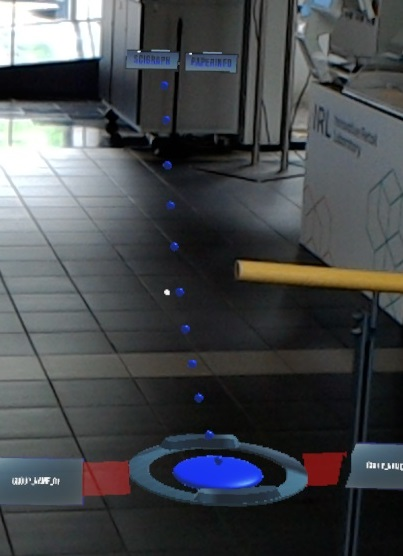
\includegraphics[width=8cm]{pov.jpg}
\caption{The Walkable Graph: Point of View}
\end{figure} \par


\subsubsection{GroupNode}
This next prefab is the previously mentioned object that spawns upon walking onto the point of view. It represents the individual group of a cluster of references. The group node prefab has no buttons and just like the point of view, fires an event by walking onto it. Being triggered like so, it spawns the reference nodes and passes them their node data.
Furthermore, lines are generated connecting the group with its reference nodes and displaying the node titles on Placard objects along the route. In this process, it destroys all other reference nodes from other groups that are active in the scene to save place. Placard objects, displaying a placeholder group name, and the group node itself can be seen in the following picture.
\clearpage

\begin{figure}[h!]
\centering
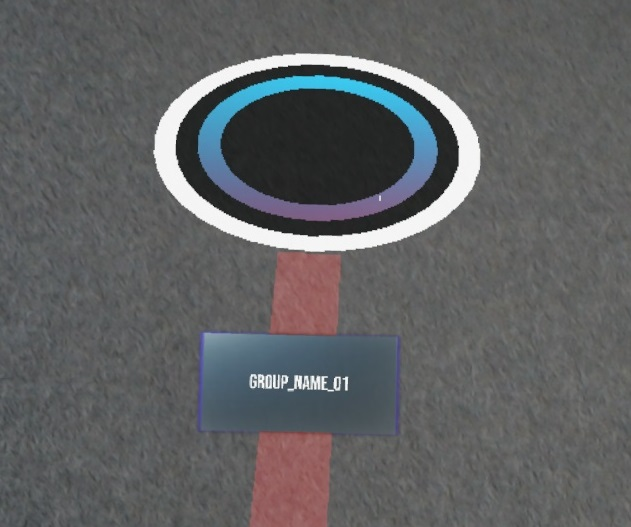
\includegraphics[width=8cm]{groupNode.jpg}
\caption{The Walkable Graph: GroupNode}
\end{figure} \par

\subsubsection{PaperNode}
The paper node prefab represents the reference node of the paper and is one of the leaves of the graph. By walking onto the paper node, all InfoPanel and ImageHolder objects of other paper nodes are hidden, to spare place. It has three buttons, the InfoPanel, SciGraph, and NewOrigin button. The InfoPanel and SciGraph buttons are utilized in the same way as it was mentioned previously. The NewOrigin button is used to create a new walkable graph that represents the paper, which the NewOrigin button belongs to.
\newline
To spare place, the beginning of the new figured walkable graph is at the same position as the recently produced point of view object. By activating the NewOrigin button completes one all the more thing, it saves every present object in an ArrayList and passes the outcome to the script appended to the main camera of the scene, called IMainCamera. In the wake of doing as such, the present objects get destroyed, and the point of view with the new XML record gets instantiated. With two extra buttons, which get created after the NewOrigin button was triggered, the past and next paper would then be able to be loaded utilizing the data put away in the IMainCamera script.
\clearpage

\begin{figure}[h!]
\centering
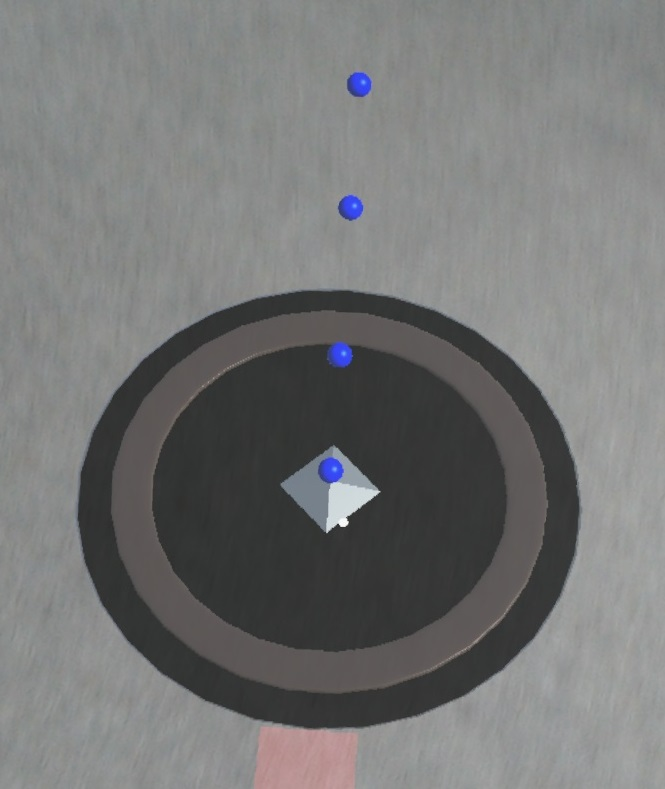
\includegraphics[width= 8cm]{paperNode.jpg}
\caption{The Walkable Graph: PaperNode}
\end{figure} \par

\subsubsection{ImageHolder}
The image holder prefab is utilized to show the SciGraph given onto a white surface. The SciGraph image gets loaded as a two-dimensional texture from the StreamingAssets folder on the HoloLens. On the off chance that the picture is absent, which can happen since the SciGraph is optional, the button of the same name is hidden. 

\subsubsection{InfoPanel}
The info panel prefab is utilized to show the paper data like title, authors, keywords, year of publishment, typology, and the abstract. 
If the textual data floods the TextMeshPro page, additional pages are created via a script and buttons are spawned to empower the user to switch between pages through an airtap gesture. In case there is no next page or previous page, the corresponding button is being hidden.
\clearpage
\begin{figure}[h!]
\centering
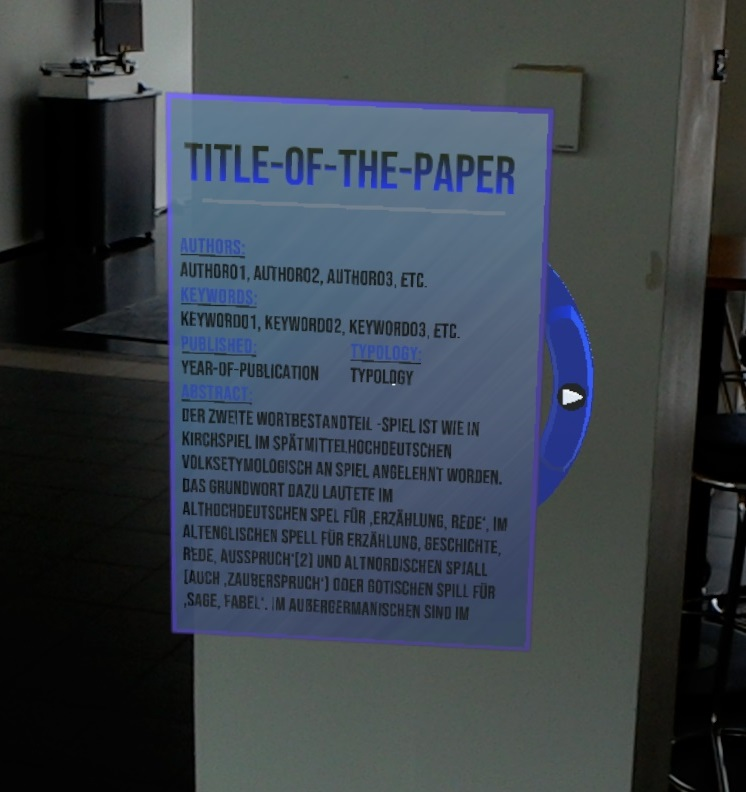
\includegraphics[width=8cm]{paperInfo.jpg}
\caption{The Walkable Graph: InfoPanel}
\end{figure}
\begin{figure}[h!]
\centering
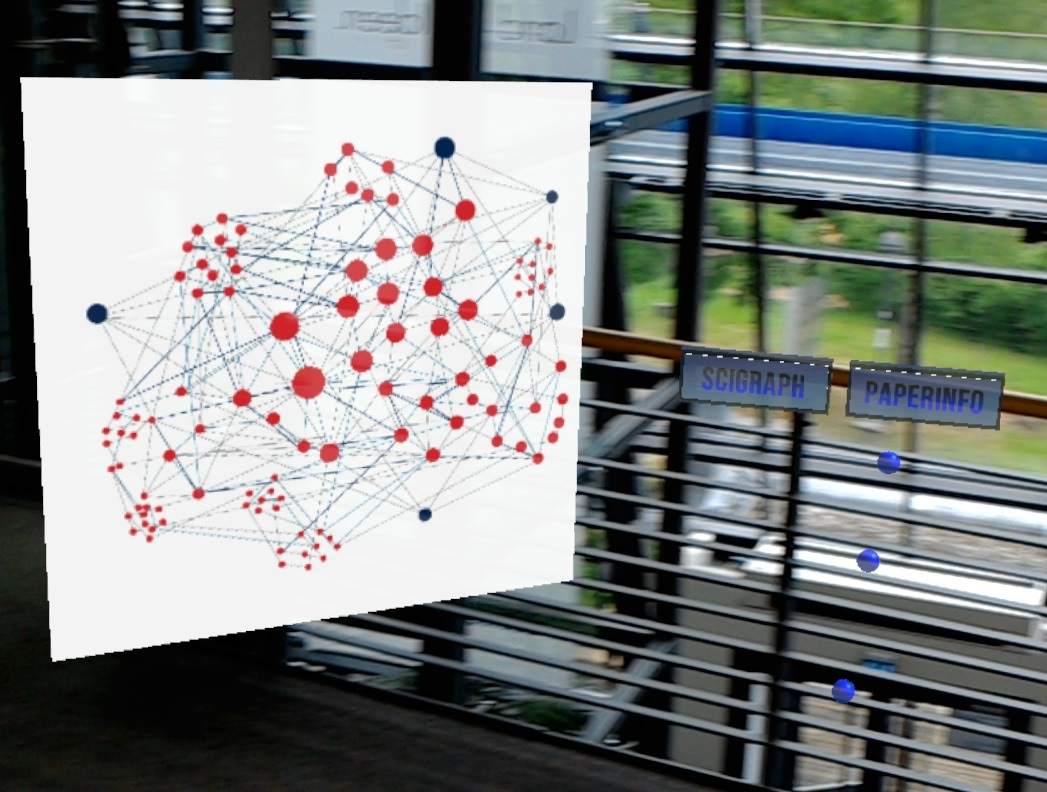
\includegraphics[width=8cm]{sciGraph.jpg}
\caption{The Walkable Graph: ImageHolder}
\end{figure}
There is no image demonstrating the button, the start menu, and line prefab explicitly since they are of minor intrigue. They can still be seen in combination with the other components of the walkable graph. The button prefab is utilized to fire an event by using an airtap gesture. At the same time, it changes its shape and shading and plays a ticking sound to give the client feedback, visually and with sound. 
\newline
The line prefab is used to direct the user from the point of view to the groups and from there further to the reference nodes, and the start menu prefab is utilized to switch among past and next papers previously visited by the user, without limitation of the depth.
\newline
The following picture shows the walkable graph, all things considered, seen from the HoloLens and closes the prefab creation area, which was a significant advance for the automated graph generation process.
\begin{figure}[h!]
\centering
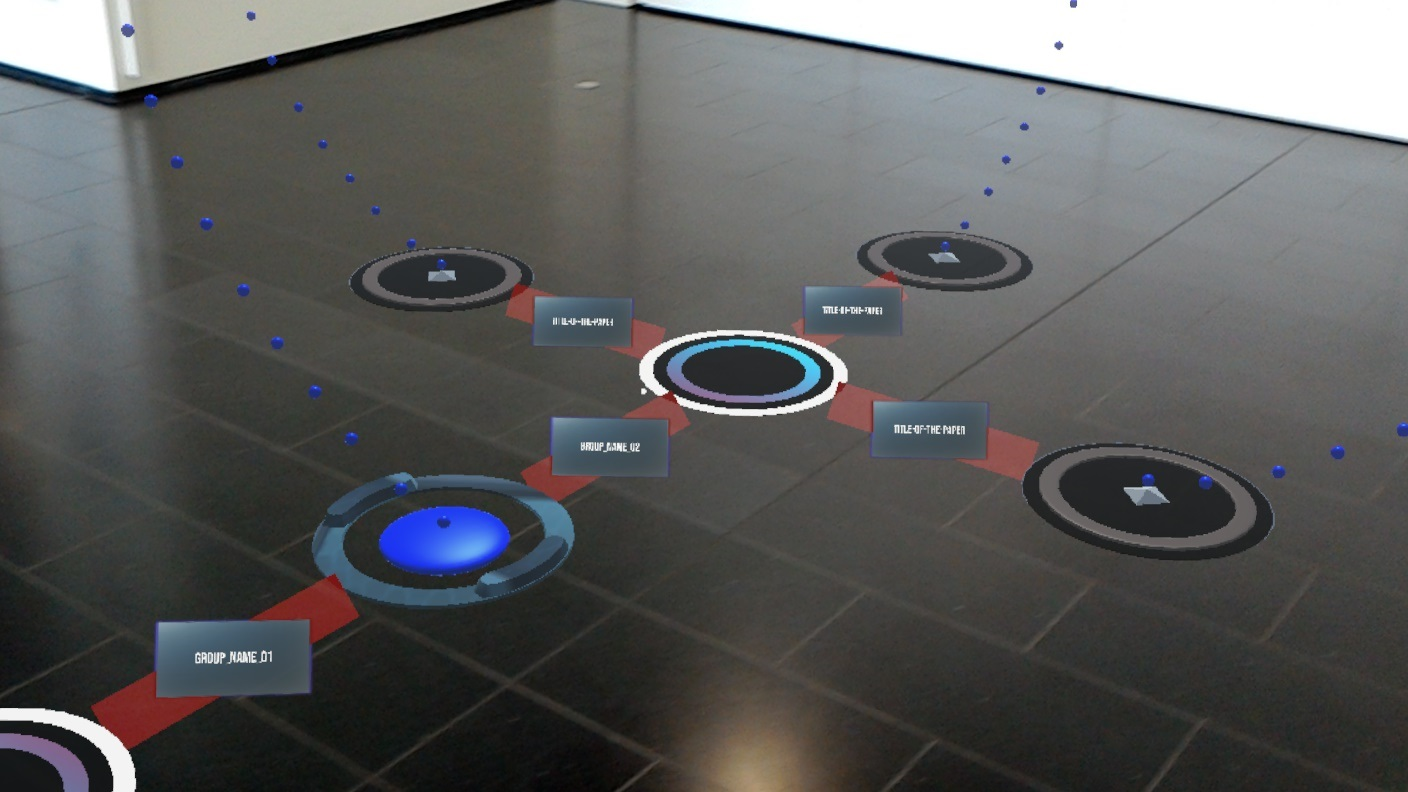
\includegraphics[width= 10cm]{graph.jpg}
\caption{The Walkable Graph: Image from HoloLens}
\end{figure} \par

\subsection{Constraints}
In this section, I am going to discuss the constraints that should be characterized, to such an extent that the walkable graph can be figured consequently, without place problems and in a symmetric manner. Since it is necessitated that the displayed system works for each measure of groups and measure of paper nodes, mathematical computations, and a requirements analysis are required. 
Achieving this, while attempting to get the base of room necessity and compute an appropriate height on which the AR contents should be displayed is the errand of this segment.
\newline
First, the problem fields are being discussed; after that, an answer to the given issues is introduced.

\subsubsection{Graph Symmetry}
The primary problem field is the symmetry of the walkable graph. Since the AR application is being used in motion, I seek to construct the walkable graph in a symmetric way, which is clear, more intuitive, and less confusing for the user contrasted with other structures.
\newline
To achieve this, I utilize a notable equation from the mathematician Leonhard Euler
\begin{equation}
e^{i \phi} = cos(\phi) + i sin(\phi), \phi \in [0, 2 \pi]
\end{equation}
called Euler's Formula. The displayed formula (1) is a portrayal of a circle with radius $ r = 1 $, computing for each input angle $\phi$ a particular point on the unit circle.
\newline
Given a particular distance from the point of view to the group nodes $d_{pov, group}$ the positions of the groups can be determined in an angle-equidistant way around the point of view by additionally fulfilling the symmetry property. Since the measure of groups is known and the distribution of the groups ought to be 360° around the point of view, the places of each separate group can be evaluated by setting the angle between two arbitrary groups to $\phi_{group} = \frac{2\pi}{m} \big(\frac{360°}{m}\big)$ while $m$ represents the number of groups. To make it more convenient for the user, I included a $\frac{\pi}{2}$ term (90°) to the resulting angle, with the end goal that the first group always spawns in front of the user. Formally speaking this means $\phi'_{group_{j}} = \phi_{group} \times j + \frac{\pi}{2} \mod 2\pi$, for $ j \in [0, (m - 1)]$.
\newline
These contemplations result in the following formula to set the places of the groups:
\begin{equation}
Pos_{group_{j}} = \Big(\cos \big(\phi'_{group_j} \big) \times d_{pov, group} , 0, \sin \big(\phi'_{group_j}\big) \times d_{pov, group} \Big)
\end{equation} while $ j \in [0, (m - 1)]$. This formula follows by inserting the angle and distance into Euler's formula.
Cause of the fact, that all instantiated objects in Unity face toward the north (z-axis), they at first as of now have a 90° rotation. Therefore, the groups itself should be rotated $\phi'_{group} \times \frac{180°}{\pi} - 90°$ further, to face the direction it was spawned too. The $ \frac{180°}{\pi}$ part represents the conversion from radians to angles.
\newline
Similar to equation (2) the positions of the paper nodes can be computed in the same way, by using an additional value, the translation of the particular group, the paper node belongs to.
Since the number of nodes is known for each group, the paper nodes can be allocated in an angle-equidistant way around the group. 
\newline
I define the length of the lines of the graph to be at least one meter, to make sure to create a reasonable graph.
With this information, an optimal angle range can be calculated so that paper nodes do not intersect with the connecting line between their group and the point of view (pov), taking up as much space as possible to place paper nodes.
For the distance between the paper node and the pov - group line at least the range $r$ of the paper node is needed, plus an additional margin of 0.1, to be save, disregarding the line thickness since it just has a width of 0.02.
With the help of the Pythagoras formula and $r = 0.25$, the angle between the paper - group line and the pov - group line, called $\alpha$, can be computed as follows:
\begin{equation*}
\alpha = \arcsin \Big(\frac{r + 0.1}{1}\Big) = \arcsin (0.35) = 20.49° \approx 22.5°
\end{equation*}
%
%
\begin{figure}[h!]
\centering
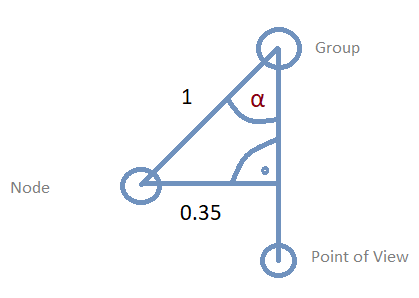
\includegraphics[width=7cm]{angle.png}
\caption{Graph Symmetry: Angle Computation for Paper Nodes}
\end{figure}
\newline
Since this angle is needed on both sides of the pov - group line, a remaining angle of 315° $\big(\frac{7\pi}{4}\big)$ can be shared by the paper nodes. 22.5° $\big(\frac{\pi}{8}\big)$ was chosen instead of 20.49° because it is better to work with, in calculations.
Shifted by $\alpha - 90° = - 67.5°$ , and further assuming the amount of nodes is $n$, the nodes start at 292.5° $\big(\frac{13\pi}{8}\big)$ and the following angles result for each node.
\begin{equation*}
\phi_{node_{i}} = \frac{13\pi}{8} + \frac{7\pi}{4(n - 1)}i \mod 2\pi, \text{for } i \in [0, (n - 1)].
\end{equation*}
In the critical case $n = 1$, where the quotient is zero, I set $\phi_{node_{1}} = \frac{\pi}{2}$, letting that one paper node be placed in front of the user.
Say the rotation of the group $k$, the paper nodes belong too, in the Unity editor is $\phi_{group_k}$, this value needs to be added to $\phi_{node_{i}}$, in more formal words $\phi'_{node_{i}} = \phi_{node_{i}} + \phi_{group_k}$. Further assuming the position of the respective group is at $(group_x, 0, group_z)$ and the distance between the group node and the paper node is $d_{group,node}$, these considerations lead to the following formula to set the positions of the paper nodes:
\begin{align*}
Pos_{Node_{i}} = \Big(\cos \big(\phi'_{node_{i}}\big) \times d_{group,node} + group_x, 0, & \\ 
\sin \big(\phi'_{node_{i}}\big) \times d_{group,node} + group_z \Big) &
\end{align*} while $ i \in [0, (n - 1)]$.
Finally, similar to the rotation of the group node itself, the paper node $i$ needs to be rotated too. Therefore, by setting the rotation to $\phi'_{node_{i}} \times \frac{180°}{\pi} - 90°$ the symmetry issue is finally solved.

\subsubsection{AR Content Placement}
Since the application "The Walkable Graph" should work for every amount of group and paper nodes given, the placement of the AR content must be planned and discussed in detail. To find a solution to this problem, it needs to be broken down into subproblems facing our situation and the desirable goals first.
The main problem is the placement of the AR content into the AR environment without objects intersecting with each other; in other words, the creating of a planar graph.
\newline
For this reason, the following subgoals are desirable:
\newline
\begin{enumerate}
    \item Find a near-optimal distance $d_{pov, group}$ from the point of view object to every other group object, such that group objects do not intersect with each other. ( 360° arrangement )
    \item Find a near-optimal distance $d_{group, node}$ from the group object to every other paper node object, such that paper node objects do not intersect with each other. ( 315° arrangement )
    \item Make sure that paper nodes do not intersect with other group objects.
\end{enumerate}
From the VR Model Preparation process the number of group nodes $m$ and the number of paper nodes $n_j$ for each respective Group Node $j = 1,..,m$ is known. Furthermore, the group objects should have a 360°, and the paper nodes a 315° arrangement.
\newline
Besides, I want the distances $d_{pov, group}$ and $d_{group, node}$ to be at least one meter long to guarantee a reasonable walkable graph and the radians of the point of view, group and paper - node circles set to $r = 0.25$. The radians of the objects can be arranged, like any other global value of the walkable graph in a script called "Config."
Since the calculations for the distance $d_{pov, group}$ will depend on the distance calculations of $d_{group, node}$ I will begin to give a solution for the subgoal (2) first.
To make sure that the paper nodes do not intersect with each other, $d_{group, node}$ must be chosen long enough such that two arbitrary paper nodes $ref_1$ and $ref_2$ have a minimal distance of $2r$ to each other. In more formal words, we need $d\big(Pos(ref_1), Pos(ref_2)\big) \ge 2r$.
\newline
To save the symmetry property, I set the number of paper nodes $n$ that I work within the following formulas, to the maximum amount of paper nodes appearing in any group. If it works for the worst case, it works for any case. It would also work to look at each group respectively but would result in way more calculations needed, complicating the issue and somewhat breaking the symmetry because the distance from group to reference node would variate from group to group.
Since its a 315° arrangement for paper nodes, the angle between two arbitrary paper nodes is $\beta = \frac{7\pi}{4(n - 1)}$. Without any loss of generality, I assume that 
\begin{equation}
Pos(ref_1) = (d_{group, node}, 0, 0)
\end{equation}
, such that the neighbor node $ref_2$ is at the following position
\begin{equation}
Pos(ref_2) = \big(d_{group, node} \times \cos(\beta), 0, d_{group, node} \times sin(\beta) \big)
\end{equation}
The distance between the two paper nodes can then be estimated with equations (3) and (4) like in the following:

\begin{align*}
d\big(Pos(ref_1), Pos(ref_2)\big) &\ge 2r \\
\Leftrightarrow \left\Vert \Big(\big(\cos(\beta) - 1 \big) \times d_{group, node} , 0, \sin(\beta) \times d_{group, node} \Big) \right\Vert_{2} &\ge 2r \\
\Leftrightarrow d_{group, node} \times \sqrt{2 - 2 \cos(\beta)} &\ge 2r \\
\Leftrightarrow d_{group, node} &\ge \frac{2r}{\sqrt{2 - 2\cos\big(\frac{7\pi}{4(n - 1)}\big)}}
\end{align*}

Since I want a minimal distance of one, we now get the following formula for the distance:
\begin{equation}
d_{group, node} = max \left(1, \left\lceil \frac{2r}{\sqrt{2 - 2\cos\big(\frac{7\pi}{4(n - 1)}}\big)} \right\rceil \right)
\end{equation}
, where $\lceil$  $\rceil$ means that the value is rounded up by two fractional digits, disregarding millimeters.
\newline
By solving subgoal (2), we are now able to solve subgoal (3) which depends on the result of the distance $d_{group, node}$ from above. The distance  $d_{pov, group}$ has to be chosen long enough, to make sure that any paper node and any group will not intersect with each other.
\newline
The worst-case scenario is delineated in the following picture, where the paper node of a group goes in a direction with a 90° angle towards the line from the pov to another group. This line represents the shortest path from group 2 to the pov - group 1 line. These considerations are only possible for $m \geq 5$, since, for $m \leq 4$ , the angle $\phi_{group} \geq \frac{\pi}{2}$, such that there can not be another 90° angle because triangles have an inner angle sum of 180° in total.
%
%
\begin{figure}[h!]
\centering
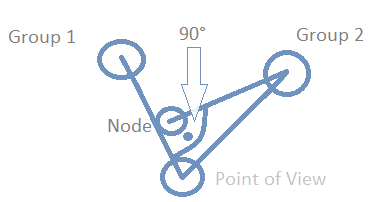
\includegraphics[width=7cm]{angle2.png}
\caption{Content Placement: Distance Computation}
\end{figure}
\newline
Since the angle between two groups is known to be $\phi_{group} = \frac{2\pi}{m}$, and the distance from the group2 to the pov - group1 line needs to be at least $d_{group, node} + 2r$, one $r$ needed for the paper node radius and one $r$ needed for the group radius, the Pythagoras formula can be used once again.
\begin{align*}
\sin(\phi_{group}) &\geq \frac{d_{group, node} + 2r}{d_{pov, group}} \\
\Leftrightarrow d_{pov, group} &\geq \frac{d_{group, node} + 2r}{\sin(\frac{2\pi}{m})}
\end{align*}
Since I want a minimal distance of one, we now get the following formula for the distance:
\begin{equation}
d_{pov, group} = max \left(1, \left\lceil \frac{d_{group, node} + 2r}{\sin(\frac{2\pi}{m})} \right\rceil \right)
\end{equation}
, where $\lceil$  $\rceil$ means again that the value is rounded up by two fractional digits, disregarding millimeters.
\newline
For the critical cases $m = 1$ and $m = 2$, where $sin(.) = 0$, I set $d_{pov, grou} = 1$, since paper nodes can not intersect with other pov - group lines in those cases.
For the case where $m = 3$ we have an angle of 120° $\big(\frac{2\pi}{3}\big)$ between the group nodes, and in the worst case scenario an angle of about 22.5° $\big(\frac{\pi}{8}\big)$ from the pov - group line to the group - paper line. With these information, the Sinussatz can be used to determine the distance $d_{pov, group}$ as follows:
\begin{align}
\frac{d_{group, node} + 2r}{\sin\big(\frac{2\pi}{3}\big)} &= \frac{d_{pov, group}}{\sin\big((180° - 120° - 22.5°) \frac{\pi}{180°}\big)} \\
d_{pov, group} &= \frac{d_{group, node} + 2r}{\sin\big(\frac{2\pi}{3}\big)} \sin\big(37.5° \frac{\pi}{180°}\big)
\end{align}
In the case $m = 4$, there is a 90° angle between the groups, and therefore the distance can be computed with Pythagoras again, as follows:
\begin{align}
\cos\big(\frac{\pi}{8}\big) &= \frac{d_{pov, group}}{d_{group, node} + 2r} \\
d_{pov, group} &= \cos\big(\frac{\pi}{8}\big) (d_{group, node} + 2r)
\end{align}
\newline
For the calculations in the cases $m = 3$ and $m = 4$ figure (17) should be taken as reference.
The remaining subgoal (1) is already satisfied by subgoal (3), since if the distance $d_{pov, group}$ is large enough between two groups and a paper node in between, it is large enough for two groups solely as well.
\newline
In conclusion, the two formulas (5) and (6), together with the edge cases (8) and (10), satisfy all the predefined subgoals and solve the placement issue for the AR content of the AR application "The Walkable Graph." In the following, I will present a table that calculates the radius needed for the walkable graph, for a given n, m and $r = 0.25$. 

\begin{table}[h]
\centering
\caption{Placement Calculations, The Walkable Graph}
\begin{tabular}{|l|l|l|l|l|} 
\hline
n & m & \textbf{$d_{group, node}$} & \textbf{$d_{pov, group}$} & max. walkable graph radius  \\ 
\hline
3          & 3          & 1                           & 1.06                        &  2.06                       \\ 
\hline
4          & 4          & 1                           & 1.39                          & 2.39                                  \\ 
\hline
5          & 5          & 1                           & 1.58                       & 2.58                               \\ 
\hline
7          & 7          & 1                           & 1.92                      & 2.92                                 \\ 
\hline
8          & 8          & 1                           & 2.12                       & 3.12                                 \\ 
\hline
10         & 10         & 1                        & 2.55                       & 3.55                              \\ 
\hline
\end{tabular}
\end{table}

Since most papers do not have more than 100 references, the maximum radius for the walkable graph should not exceed a range of 3.55 meters. All the calculations are based on Unity units, but since one Unity unit translates to one real-world meter, the estimates hold.

\subsubsection{Height Allocation}
The last constraint that should be tended to is the height allocation. Since it is alluring that the AR application "The Walkable Graph" does indeed generate walkable graphs on the floor level, no matter how tall the user is or where the application is being used, this issue should be additionally tended to. 
A few methodologies are accessible in the Microsoft HoloToolkit software I utilized all through the execution to assemble the AR application "The Walkable Graph." 
Since the Microsoft HoloLens can reason about the real-world around the user, it can likewise compute at which level the floor is.
The system I used to decide the floor height, is by utilizing purported Spatial Mapping. Spatial mapping puts a wireframe mesh on the real-world surface in the environment around the HoloLens, enabling developers to make a persuading MR experience. This mesh comprises a set of red triangles, the more triangles, the more exact the mesh is laid onto the surface. For this task, I used a mesh consisting of 500 triangles per square meter. By combining the real world with the virtual world and using Spatial Mapping, holograms of AR applications appear to be more genuine and line up with user desires more optimally, by conveying a natural, authentic experience.  \footnote{According to Microsoft Documentation \cite{mapping}}
The spatial mapping comprises of two essential object types, in particular, the Spatial Surface Observer and the Spatial Surface. With these instruments, I computed the surfaces around the user of the AR application "The Walkable Graph" by laying the mesh of triangles around the environment.
\newline
After the meshes are laid onto the environment, a technique called Spatial Processing is utilized. With this technique, it is conceivable to combine the meshes to surfaces. Each surface observer, which is part of the Spatial Processing technique, can compute different detached spatial surfaces,  and finally, put them together. Finally, a section step is required, since surface meshes frequently overlay each other somewhat. 
\newline
I utilized Spatial Processing to combine the meshes, explicitly the floors, roof, and walls mesh surface. Together with the SurfaceMeshesToPlanes script that is incorporated into the HoloToolkit, this gives me the information about the environment, needed to decide the floor level. 
The least Y - value vertices indicate the floor height.
The entire procedure portrayed here takes only three seconds altogether, which is a reasonable time for the user to hang tight for.\footnote{According to Talesfromtherift \cite{understanding}}
\newline
This mesh can be seen in the following picture:
\begin{figure}[h!]
\centering
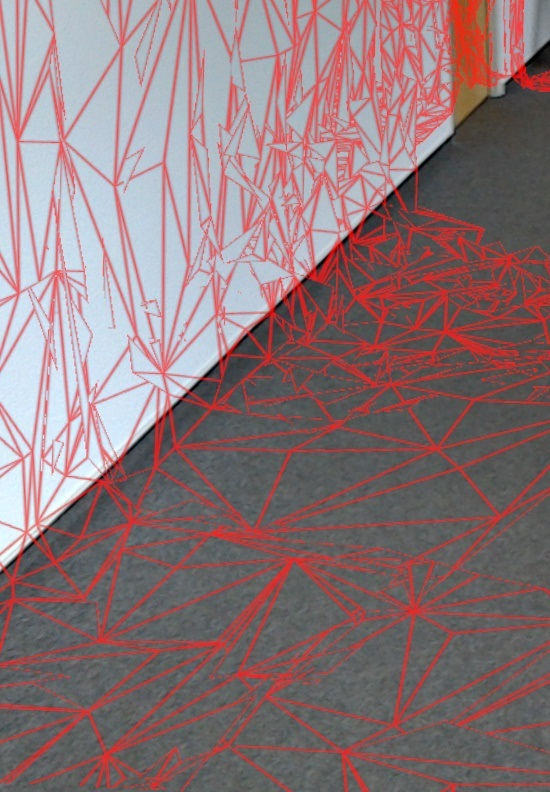
\includegraphics[width= 7cm, height = 5cm]{redmesh.jpg}
\caption{Microsoft HoloLens: Spatial Mesh}
\end{figure}
\newline
Spatial Processing is to a higher degree viewed as a part-solution, than a full solution. Nevertheless, Spatial Processing satisfies the requirement for the picked use case. The other plausibility to accomplish a similar outcome is to utilize Spatial Understanding, which can be considered as a full solution.
\newline
Spatial Understanding opens far and away superior and more exact meshes, and surface discovery than Spatial Processing can accomplish to do. With this, even the identification of obstacles in the room is possible. Moreover, holograms can be placed on sufficiently large floor surfaces or tables naturally. \footnote{According to Talesfromtherift \cite{understanding}}
\newline
Since Spatial Understanding needs the space to be pre-scanned in a slow and time-consuming procedure, I did not utilize this technique in my prototype execution.
Especially for evaluation reasons, it is desirable to have a fast walkable graph computation and an uncomplicated process for the user.
The following picture demonstrates the Spatial Understanding technique in action:
\begin{figure}[h!]
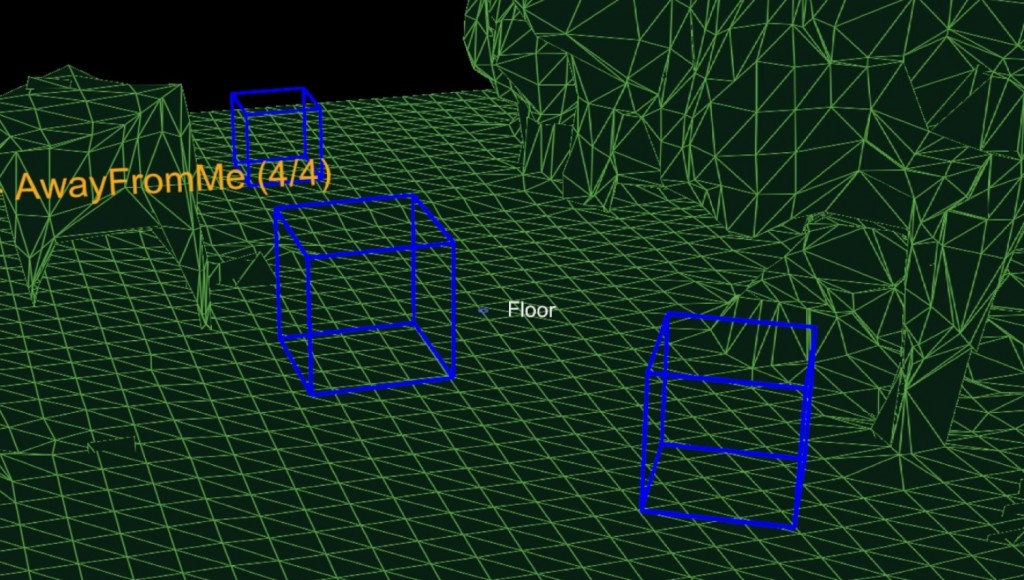
\includegraphics[width= 10 cm]{understanding.jpg}
\centering
\caption{Microsoft HoloLens: Spatial Understanding \cite{understanding}}
\end{figure}
\newline
Since a satisfying answer for every one of the constraints was given, every one of the prerequisites is fulfilled, and the automated graph generation procedure can begin.


%%% Tools %%%
\subsection{Tools}

\subsubsection{Unity 3D}
The underlying software utilized all through the entire development of the exhibited model "The Walkable Graph" is the software called Unity. It is one of the world's driving, real-time creation platform. Unity is utilized to make half of the world's games; practically the other half is made through UnrealEngine. Unity's real-time platform, controlled by instruments and administrations, offer excellent potential outcomes for game designers, and developers crosswise over enterprises and applications. All through my usage procedure, I utilized the free form of Unity for the development of the prototype.
\newline
It is a content creation motor that empowers the client to create applications for several platforms, including the \ac{UWP}, which is the platform utilized for HoloLens application development. It is likewise the platform, which made the creation of prefabs and the automation of the AR content creation conceivable. The scripts, which are needed to implement particular behavior of the AR objects are written in C\#.\footnote{According to Unity Documentation \cite{unity2}}

\subsubsection{Visual Studio Code}
Visual Studio Code is a lightweight yet ground-breaking source-code editorial manager which is accessible for Windows, macOS, and Linux. Throughout my thesis, I am utilizing this editor as my C\# code editor, since it is user-friendly and easy to get familiar with. 
It further supports programming languages like JavaScript, TypeScript, Node.js and many more and has a system of expansions, for customizations.
\newline
It likewise bolsters runtime engines like Unity and aides to debug MonoBehavior scripts that are utilized to implement events occurring in Unity and the AR application "The Walkable Graph." It furthermore provides the developer with code snippets, which fasten the whole development process. \footnote{According to Visual Studio Code Documentation \cite{vscode}} 

\subsubsection{Visual Studio Community 2017}
The Visual Studio IDE is an innovative platform that can be used to alter, troubleshoot, and develop code, and afterward distribute an application. 
An IDE is a component rich program that can be utilized for developing code.
Well beyond the standard debugger that most IDEs give, Visual Studio incorporates compilers, graphical design tools, and a lot more highlights to facilitate the software development process. In the case of my bachelor thesis, I used this IDE to deploy the build AR application, "The Walkable Graph" onto the HoloLens Emulator or the real HoloLens device. I used the free version of this software called Visual Studio Community. \footnote{According to Visual Studio Documentation \cite{vsstudio}}

\subsubsection{Mixed Reality Toolkit (MRTK)}
There are plenty of frameworks that enable AR development, but since the MRTK is the most suggested framework by Microsoft, it is the framework I chose.
The MRTK gives a lot of fundamental components and highlights to quicken VR and AR application development in Unity. It is a Microsoft driven open source project, to help developers with pre-made prefabs and valuable contents. The MRTK empowers fast prototyping through in-editorial simulation that enables the developer to see changes quickly, while additionally giving fundamental building blocks for Unity development on HoloLens, Windows Mixed Reality, and OpenVR. The feature regions of this product incorporate the input system, gestures for the HoloLens, voice commanding, gaze, teleportation, and spatial understanding, and some more. The variant I used to execute "The Walkable Graph" is the MRTK v1 release, since the most recent adaptation is not running on my system. The following picture from their GitHub repository demonstrates a couple of the pre-made prefabs:\footnote{According to MRTK on GitHub \cite{mrtk}}
\clearpage

\begin{figure}[h]
\centering
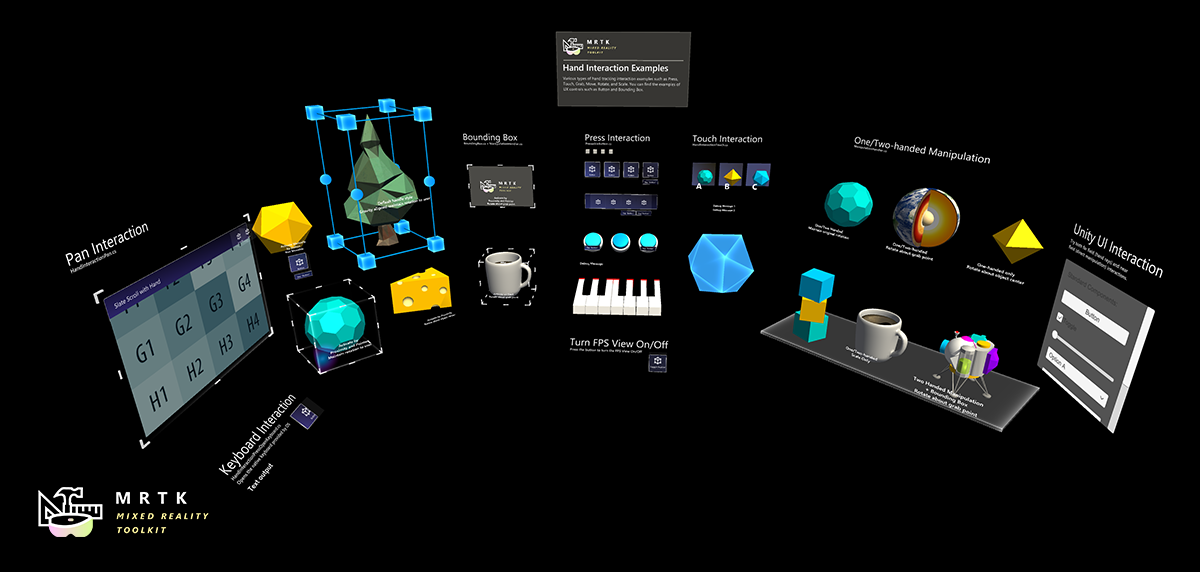
\includegraphics[width=10cm]{mrtk.png}
\caption{MRTK Prefab Examples \cite{mrtk}}
\end{figure} \par


\subsubsection{Microsoft HoloLens Emulator}
The HoloLens Emulator enables the developer to test holographic applications on the computer without a physical HoloLens and accompanies the HoloLens development toolset. The emulator utilizes the Hyper-V virtual machine, which is an additional feature of Windows 10 and needs to be activated in developer mode beforehand. The gestures, which are usually recognized by the sensors of the physical device, need to be reenacted utilizing the developer's console, mouse, or Xbox controller.
Applications do not need to be altered to be able to run on the emulator and therefore, do not have a clue about that they are not running on a genuine HoloLens. For the development of the prototype "The Walkable Graph," I used the HoloLens Emulator to test and debug the AR application. The emulator allowed me to make changes to the AR application from at home, without the need to use the physical device. The version I used while implementation is the HoloLens Emulator build 10.0.14393.1358, which is not the latest release, but for me, it was the fastest running..\footnote{According to HoloLens Emulator Documentation \cite{emulator}}

\subsubsection{Microsoft HoloLens}
The HoloLens is an AR device developed by Microsoft, which is the world's first completely untethered holographic head-mounted computer.
It can reason about the world around the user and recognize gestures that are performed by the user in front of the sensors, engaging the user in new ways.
HoloLens mixes cutting-edge optics and sensors to convey 3D visualizations stuck to this present reality around the user. 
There are two variants of the HoloLens, which can be bought, the developer edition and the consumer edition.
\newline
The development of the AR application, "The Walkable Graph" was specifically targeted for this fascinating device. In my case, I used the HoloLens 1st Gen Developer Edition from the DFKI Saarbrücken. A picture of the HoloLens device and the most typically used gesture to interact with AR content in the mixed reality environment follows.\footnote{According to HoloLens Documentation \cite{holodoc}}

\begin{figure}[h]
\centering
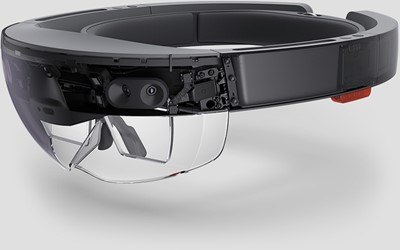
\includegraphics[width=7cm]{holodevice.jpg}
\caption{Microsoft HoloLens: Device \cite{holodoc}}
\end{figure} \par

\begin{figure}[h]
\centering
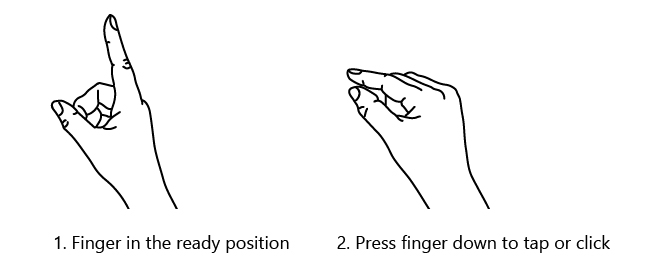
\includegraphics[width=10cm]{airtap.png}
\caption{Microsoft HoloLens: Selection-Gesture \cite{holodoc2}}
\end{figure} \par


\subsubsection{Programming Language C\#}
C\# is a universally useful programming language that was developed around 2000 by Microsoft. Initially planned by  Anders H. and later on approved as a standard by ECMA, C\# evolved to a widely used object-oriented programming language. As of right now, Mads T. drives its development group. The latest version is C\# 7.3, which was discharged in 2018 close by Visual Studio 2017 adaptation 15.7.2. Every one of the scripts in Unity that handle a wide range of events and process the walkable graph is written in C\# and get later on, with the deployment to the HoloLens, converted into C++. C\# is an object-oriented programming language, but C \# further includes support for component-oriented programming. It also shares a ton with the Java programming language. \footnote{According to C\# Documentation \cite{csharp}}

\subsubsection{TextMeshPro}
TextMeshPro is an Asset - Bundle, which I have utilized all through the execution of  "The Walkable Graph." This Asset - Bundle utilizes advanced content rendering techniques to convey significant visual quality enhancements, adaptability in content styling, and texture. Furthermore, it gives improved power over content organizing and format and therefore, brings State-Of-The-Art content rendering to Unity.\footnote{According to TextMeshPro - Unity Asset Store \cite{tmpro}}

\clearpage
\section{Evaluation Plan}
This section seeks to give an assessment plan for further examination and evaluation of the implemented proof-­of-­concept prototype," The Walkable Graph." Consequently, this area will elucidate what the prototype was initially worked for, concerning that information it will be talked about which factors do exist that are important to be assessed and a proposition on how they ought to be assessed in a later research thesis. Further, factors that are identified with the thematic, however, do not address the thesis objective straightforwardly are also examined.
\newline
The prototypical execution of the AR application "The Walkable Graph" was built to give a response to the research question of this thesis, which looks for after the automatization of AR content in an AR environment, for this situation explicitly the automated graph generation in an AR environment.
Since the automated graph generation is the central purpose of this thesis, it should be assessed, and consequently, assessment factors concerning that thematic should be analyzed.
\newline
% Variables %
% Automatization vs Manual Approach, Computational Time %
A conceivable evaluation variable may be the time expected to make the walkable graph by hand contrasted with the automated approach. Since the focal point of automation depends on the way that the development time and effort of such an AR application can be diminished, this evaluation variable is of intrigue, for the most part since development time decrease results in a vast expense reduce.
\newline
These considerations lead to the following evaluation variable.
\begin{itemize}[leftmargin=2cm]
    \item [\textbf{V:}] The automated approach compared to the manual one, concerning development time and effort.
\end{itemize}
% Additional Variables%
In an, all the further sense a couple of more assessment factors may be of intrigue, regardless of whether they are not legitimately related to the research questions this thesis inspected. For instance, the information memory of the user of the AR application, "The Walkable Graph." 
\newline
% AR Approach vs. Printed/ Digital Approach, Memory Enhancement %
It could be of significant interest to explore whether the information memory of the user of the AR application was enhanced or not, contrasted with the regular perusing of the academic paper, may it be in the paper - or digital form. Just like it was previously discussed in the Related Work section, it is expected to have a better outcome contrasted with the conventional MOL technique, or the MOL technique performed in a virtual environment.
\newline
\newline
Nevertheless, the main variable of this thesis is the automation of content creation.
To evaluate $V$, particular scientific papers, preferably with different amount of text, need to be selected and the time building a walkable graph by hand in the Unity IDE be compared to the automatized approach. It is expected that the automated approach performs better than the manual approach, concerning precision, accuracy, and the time needed, to compute the walkable graph out of scientific papers.
\newline
Lastly, each participant that utilized the AR application should be evaluated through a standard Nasa-TLX questionnaire. Evaluating the tests will give an insight into how much mental, physical, and temporal effort was demanded by the application and how the overall performance was.

\clearpage
\section{Conclusion}

This section closes up this bachelor thesis, by outlining outcomes, and my work all through it. Furthermore, the research question, charac­terized in an earlier section, will be tended to yet again and analyzed, whether the
research goal was hit satisfyingly enough or not. Lastly, further advancements
and open research issues will be talked about.

\subsection{Summary}

First, an introduction was presented to motivate the reader into the AR topic, to present and discuss the research question and goal, and clarify what kind of methodology is being used.
Next on, related works were presented to build the base knowledge for the issue field, determining the limitations of previous work in this research area, and by doing so, differentiating this thesis from others and making sure that the presented work is beyond state of the art. In the next section, the development approach for the AR application was talked about, while addressing the concept of the implementation, the design process that was put into it, how the VR Model is supposed to be built and how the object creation and information processing works, that are needed to build the walkable graph.
\newline
After that, the development of the prototype "The Walkable Graph" was discussed in more detail in the Implementation section of this thesis. The Implementation section addressed the Unity Prefab Creation process, of all the parts needed for the walkable graph, and the predefined constraints - the symmetry issue, the placement issue and the height issue, which needed to be solved, such that the walkable graph would be flexible with the number of groups and nodes that it was used with.
\newline
Since the AR application is used, with the user being in motion, a more intuitive and less confusing structure for the walkable graph is needed.
This so-called symmetry issue was solved by calculating the locations of every group and corresponding reference nodes. The result of these calculations are presented in the following two formulas:

\begin{align*}
Pos_{group_{j}} = \Big(\cos \big(\phi'_{group_j} \big) \times d_{pov, group} , 0, & \\
\sin \big(\phi'_{group_j}\big) \times d_{pov, group} \Big) &
\end{align*} while $ j \in [0, (m - 1)]$, $m$ is the number of groups and $\phi'_{group_{j}} = \phi_{group} \times j + \frac{\pi}{2} \mod 2\pi$.

\begin{align*}
Pos_{Node_{i}} = \Big(\cos \big(\phi'_{node_{i}}\big) \times d_{group,node} + group_x, 0, & \\ 
\sin \big(\phi'_{node_{i}}\big) \times d_{group,node} + group_z \Big) &
\end{align*} while $ i \in [0, (n - 1)]$, $n$ is the maximum number of nodes, $group_x \text{ and } group_z$ the x and z position of the group this reference node belongs to and $\phi_{node_{i}} = \frac{13\pi}{8} + \frac{7\pi}{4(n - 1)}i \mod 2\pi$. Furthermore, $\phi'_{node_{i}} = \phi_{node_{i}} + \phi_{group_k}$, while $group_k$ represents the group, the paper node belongs too.
\newline
Since there cannot be any object intersections in the AR environment, the walkable graphs need to be computed to be a planar graph. Taking as less space as possible, counted in diameters, the following two formulas were derived for the distance estimations for the walkable graph:
\newline
The distance from the point of view to any group node can be computed as follows:
\begin{equation}
d_{pov, group} = max \left(1, \left\lceil \frac{d_{group, node} + 2r}{\sin(\frac{2\pi}{m})} \right\rceil \right)
\end{equation}
, where $\lceil$  $\rceil$ means that the value is rounded up by two fractional digits, disregarding millimeters.
\newline
The distance from the group node to any reference node can be computed as follows:
\begin{equation}
d_{group, node} = max \left(1, \left\lceil \frac{2r}{\sqrt{2 - 2\cos\big(\frac{7\pi}{4(n - 1)}}\big)} \right\rceil \right)
\end{equation}
, where $\lceil$  $\rceil$ means again that the value is rounded up by two fractional digits, disregarding millimeters.
\newline
Moreover, the target of the height issue it was, to compute the height at which the walkable graph can be laid on the floor, which was solved by utilizing Spatial Processing.
\newline
The next section, after that, called Tools, mentions all the 3rd party software that was used throughout the development of the AR application.
As this thesis pursues the "Prototyping" methodology, the objective of the thesis was to develop a prototype called "The Walkable Graph" that can be utilized as a proof-of-concept to demonstrate that automated AR content creation is indeed conceivable.
\newline
Since this previously presented prototype automatically generates walkable graphs as AR content in an AR environment which can be observed with the Microsoft HoloLens and extracts essential data out of print media through NLP, it fulfills the predefined research goal satisfyingly.
The latter evaluation is expected to also come to this conclusion.


\subsection{Outlook}
Since this is a bachelor thesis, the assessment of the introduced proof-of-concept prototype "The Walkable Graph" must be tended to in a later master thesis. The assessment plan in an anterior segment was made to give help for this process.
\newline
In the following, I am going to address the limitations this thesis has since no research work is 100\% confinements free. The first and most evident confinement of this thesis is the original use case for this AR application. The application can be utilized to empower the reader of scholarly papers to get additional data concerning the paper and its references in the form of AR content. To achieve this undertaking, an AR application called "The Walkable Graph" was developed in participation with Springer Nature to show the said AR content in an AR environment, explicitly as a walkable graph.
The limitation lies in the fact that the created graph depends on the data extracted by NLP. Since various data extricated by NLP results in various XML records being made and along these lines perhaps different prefabs being vital, that need to be pre-fabricated.
\newline
"The Walkable Graph" was built very adaptable, with the end goal that new XML - schemes will not influence an excessive amount of code reworking, however regardless it breaks the automation sense behind it. The following limitation of this thesis depends on the arrangement of the objects in the environment. Regardless of whether a few considerations were put into that in an anterior section, it is as yet not an ideal arrangement, since, despite everything, it takes a ton of places if the paper being registered as a walkable graph has near or over 100 references. 
The user needs a room that has roughly six meters distance across, which is just a lot for the most common rooms.
\newline
There would be some standardization required for every single scholarly paper to overcome the first limitation.
Standardization of academic papers would ensure superior outcomes concerning the content mining process done by NLP. Next on, each conceivable data of interest ought to be extracted and an XML - scheme ought to be built up that contains every one of these components with perhaps optional entries for them. Similarly, all prefabs for the various components should be made previously.
This would, to some degree, solve the main issue, while it would be a ton of extra work and still be a solution only for the scholarly papers exclusively. The positioning issue could be additionally improved by empowering the user to teleport in the AR environment to a particular node while standing still at his location. This, be that as it may, would break the entire idea behind "The Walkable Graph" since there would be no more walking included.
\newline
Another possibility would be, to enable the user to switch groups, and only make one group visible once, at a time, this would at least half the place expense. This approach was not taken, since the original concept shows a graph with all the groups and nodes at once, yet could be examined in later work.
\clearpage


	\end{normalsize}
\end{justify}
\pagestyle{plain}
%%% TEXTTEIL ENDE %%%





%%% Literaturverzeichnis %%%
	\clearpage
	\pagenumbering{Roman}
	\setcounter{page}{\thesavepage}
	\phantomsection
	\bibliographystyle{plain}
	\bibliography{literatur}
	\clearpage
%%% Literaturverzeichnis END %%%



%%% Eidesstaatliche Erklärung %%%
	\phantomsection
	\addcontentsline{toc}{section}{Statement in Lieu of an Oath}
	\begin{centering}
	\Large{\textbf{Eidensstattliche Erklärung}} \par
	\end{centering}
	\normalsize{\justify{Ich erkläre hiermit an Eides Statt, dass ich die vorliegende Arbeit selbständig verfasst und keine anderen als die angegebenen Quellen und Hilfsmittel verwendet habe.}} \par
	\vspace{\baselineskip}
	\begin{centering}
	\Large{\textbf{Statement in Lieu of an Oath}} \par
	\end{centering}
	\normalsize{\justify{I hereby confirm that I have written this Thesis on my own and that I have not used any other media or materials than the ones referred to in this thesis.}} \par
	\vspace{\baselineskip}
	\vspace{\baselineskip}
	\vspace{\baselineskip}
	\vspace{\baselineskip}
	\begin{centering}
	\Large{\textbf{Einverständniserklärung}} \par
	\end{centering}
	\normalsize{\justify{Ich bin damit einverstanden, dass meine (bestandene) Arbeit in beiden Versionen in die Bibliothek der Informatik aufgenommen und damit veröffentlicht wird.}} \par
	\vspace{\baselineskip}
	\begin{centering}
	\Large{\textbf{Declaration of Consent}} \par
	\end{centering}
	\normalsize{\justify{I agree to make both versions of my thesis (with a passing grade) accessible to the public by having them added to the library of the Computer Science Department.}} \par
	\vspace{\baselineskip}
	\vspace{\baselineskip}
	\vspace{\baselineskip}
	\vspace{\baselineskip}
	\vspace{\baselineskip}
	\begin{justify}
	Saarbrücken, \SignatureAndDate{        (Datum/Date)}
	\end{justify}
%%% Eidesstaatliche Erklärung END %%%



\end{document}